\documentclass[letterpaper,12pt]{article}
\usepackage[utf8]{inputenc}
\usepackage[english]{babel}
\usepackage{graphicx}
\usepackage{amsmath}
\usepackage{amssymb}
\usepackage[margin=0.75in]{geometry}
\usepackage{chngcntr}
\usepackage{caption}
\usepackage{fancyhdr}
\usepackage{placeins}

% Adjust the header height
\setlength{\headheight}{14.5pt}
\addtolength{\topmargin}{2.5pt}
\setlength{\parskip}{1em}

% Configure section and subsection numbering
\renewcommand{\thesection}{6.\arabic{section}}
\renewcommand{\thesubsection}{6.\arabic{section}.\arabic{subsection}}

% Redefine figure counter
\captionsetup[figure]{labelformat=empty} % Avoid automatic numbering
\captionsetup[table]{labelformat=empty} % Avoid automatic numbering

% Configure fancyhdr
\pagestyle{fancy}
\fancyhf{}
\fancyhead[L]{Chapter 6}
\fancyhead[R]{\thepage}
\fancyfoot[C]{}

\title{Two-Level Voltage Source Inverter}
\author{}
\date{}

\begin{document}
\setcounter{page}{95}

\maketitle
\thispagestyle{fancy} % Apply fancyhdr style to the first page

\section{Introduction}
The primary function of a voltage source inverter (VSI) is to convert a fixed dc voltage to a three-phase ac voltage with variable amplitude and frequency. A simplified circuit diagram for a two-level voltage source inverter for high-power medium-voltage applications is shown in Fig. 6.1-1. The inverter is composed of six group of active switches, $S_1$ to $S_6$, with a free-wheeling diode in parallel with each switch. Depending on the dc operating voltage of the inverter, each switch group consists of two or more IGBT or GCT switching devices connected in series.

This chapter focuses on pulse width modulation (PWM) schemes for the high-power two-level inverter, where the device switching frequency is normally below 1 kHz. A carrier-based sinusoidal PWM (SPWM) scheme is reviewed, followed by a detailed analysis on space vector modulation (SVM) algorithms. The conventional SVM scheme usually generates both even- and odd-order harmonics voltages. The mechanism of even-order harmonic generation is analyzed, and a modified SVM scheme for even-order harmonic elimination is presented.

\section{Sinusoidal PWM}
\subsection{Modulation Scheme}
The principle of the sinusoidal PWM scheme for the two-level inverter is illustrated in Fig. 6.2-1, where $v_{m_a}$, $v_{m_b}$, and $v_{m_c}$ are the three-phase sinusoidal modulating waves and $v_{cr}$ is the triangular carrier wave. The fundamental-frequency component in the inverter output voltage can be controlled by amplitude modulation index
\[
	m_a = \frac{\bar{v}_m}{\bar{v}_{cr}}
\]

\begin{figure}[h]
	\centering
	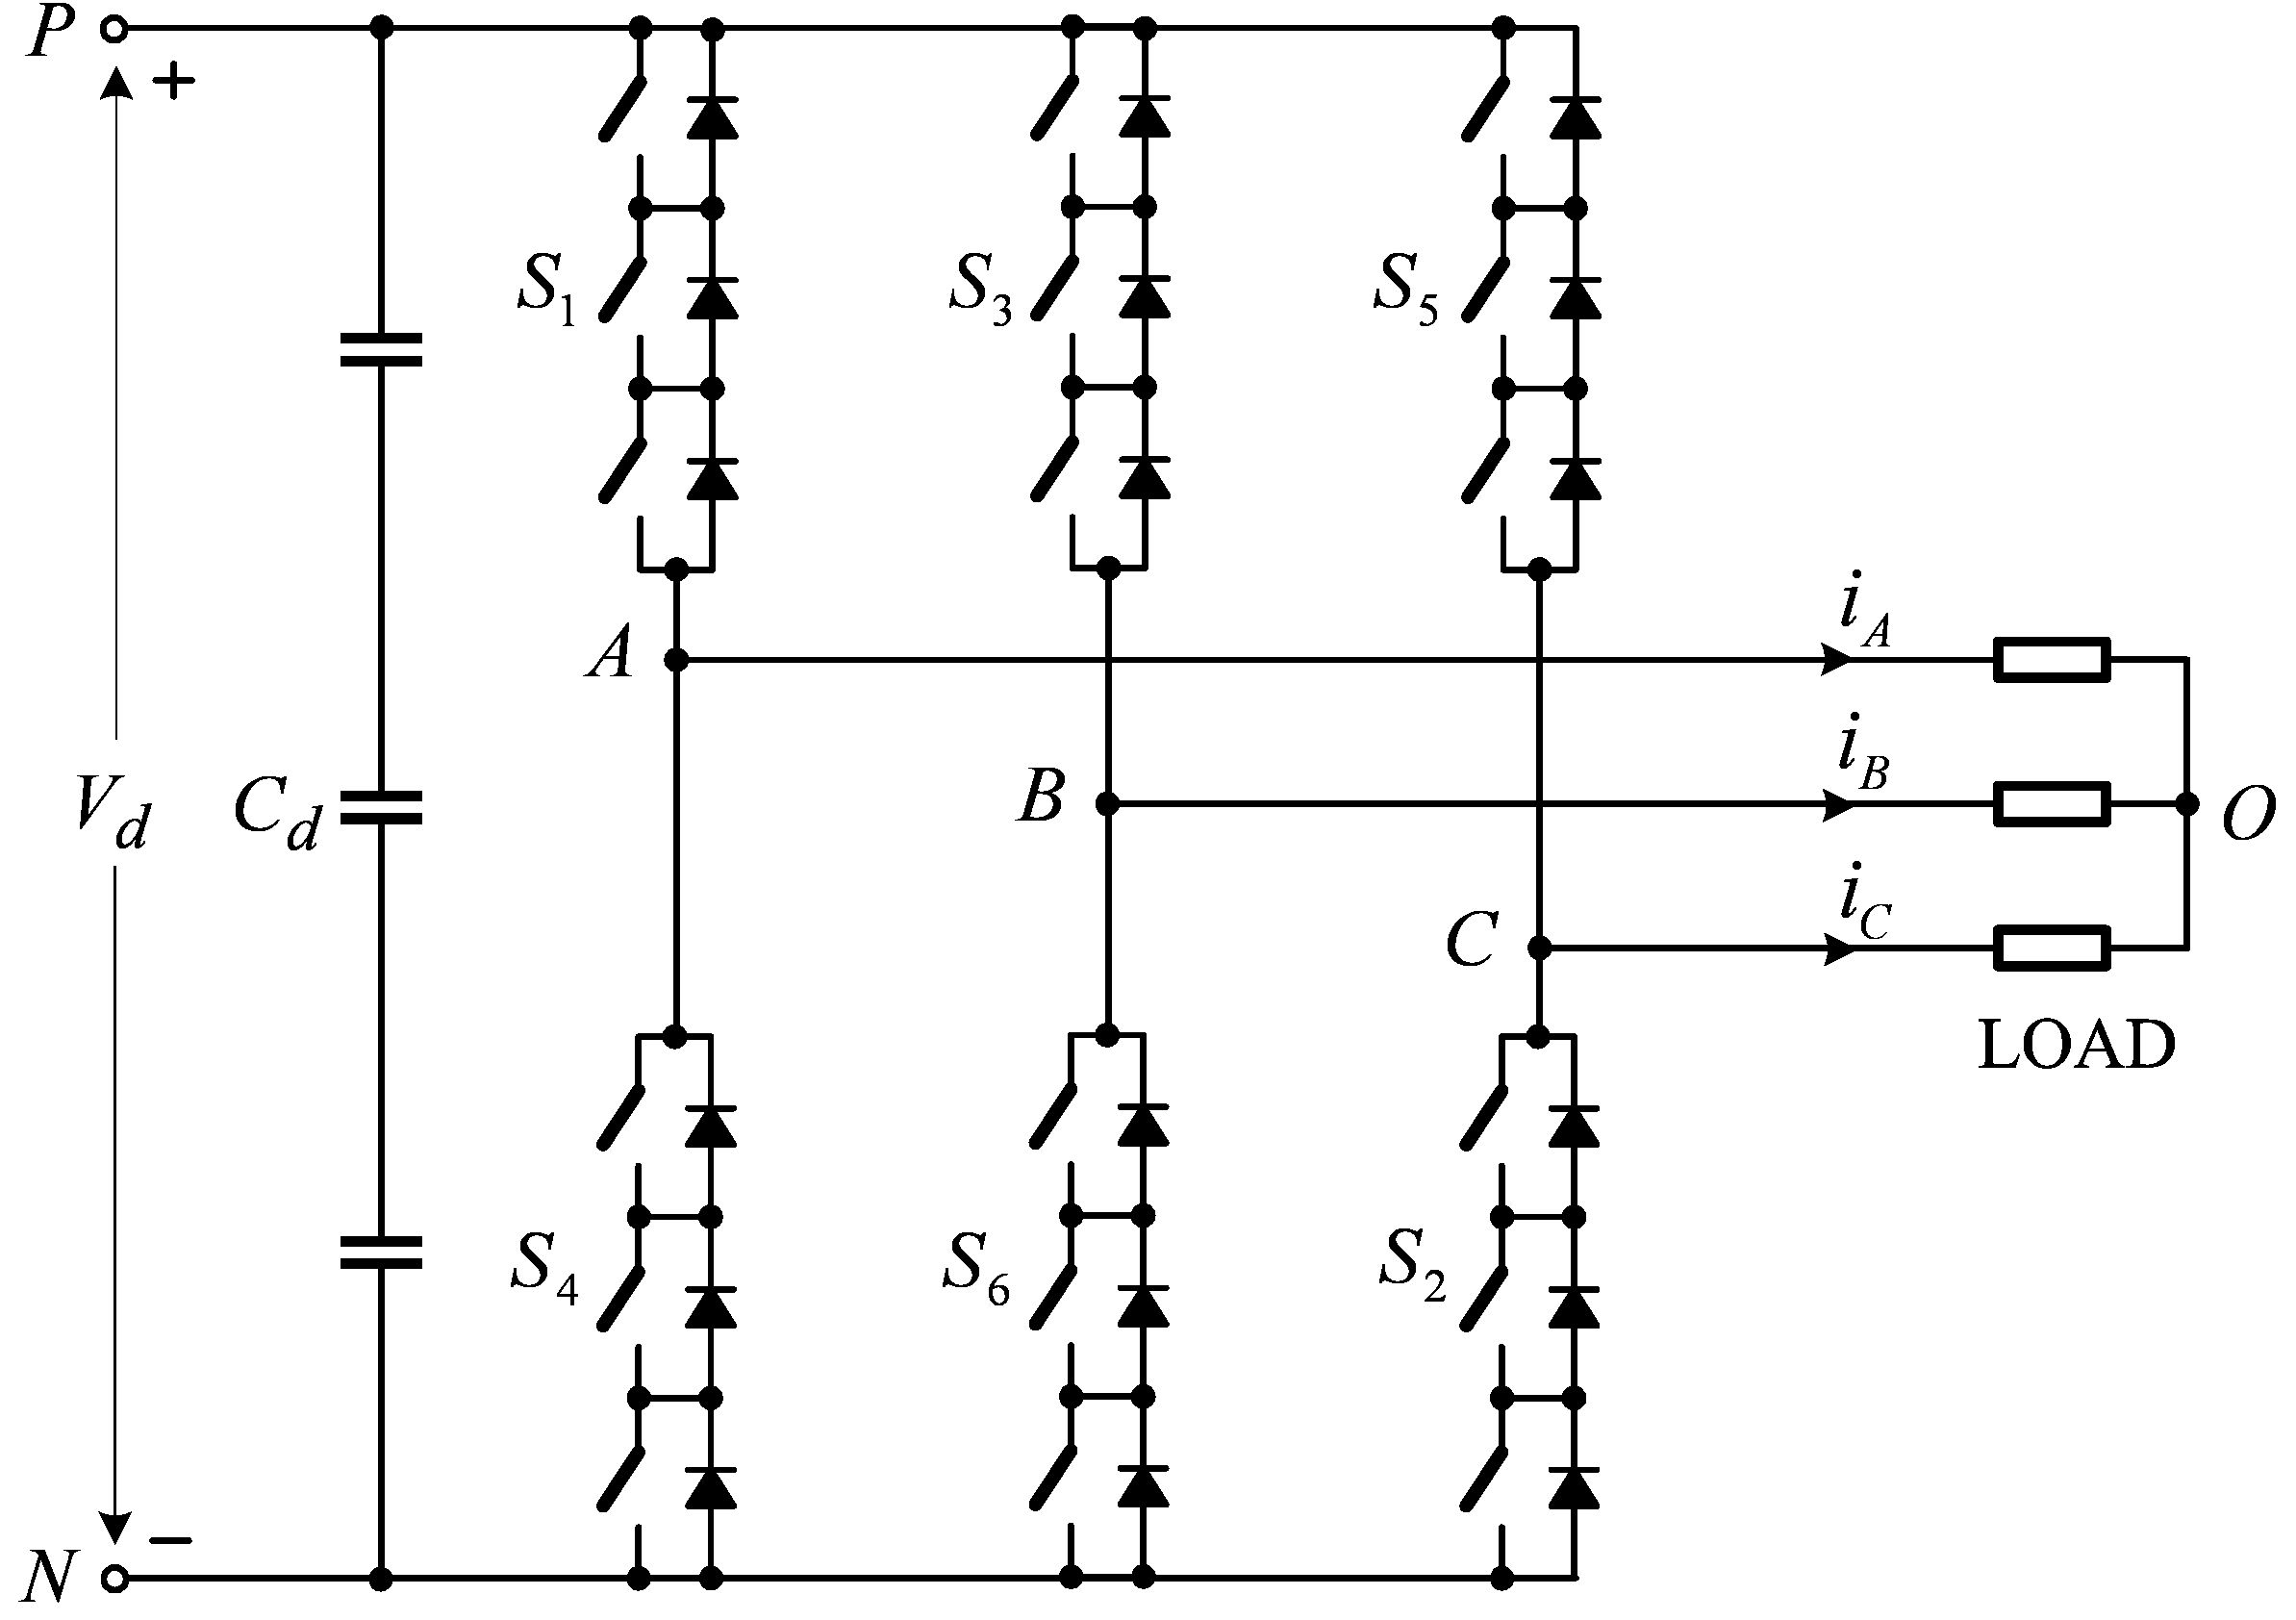
\includegraphics[width=0.5\textheight]{graficos/img61.jpg}
	\caption{Figure 6.1-1 Simplified two-level inverter for high-power applications.}
\end{figure}
\FloatBarrier

\begin{figure}[h]
	\centering
	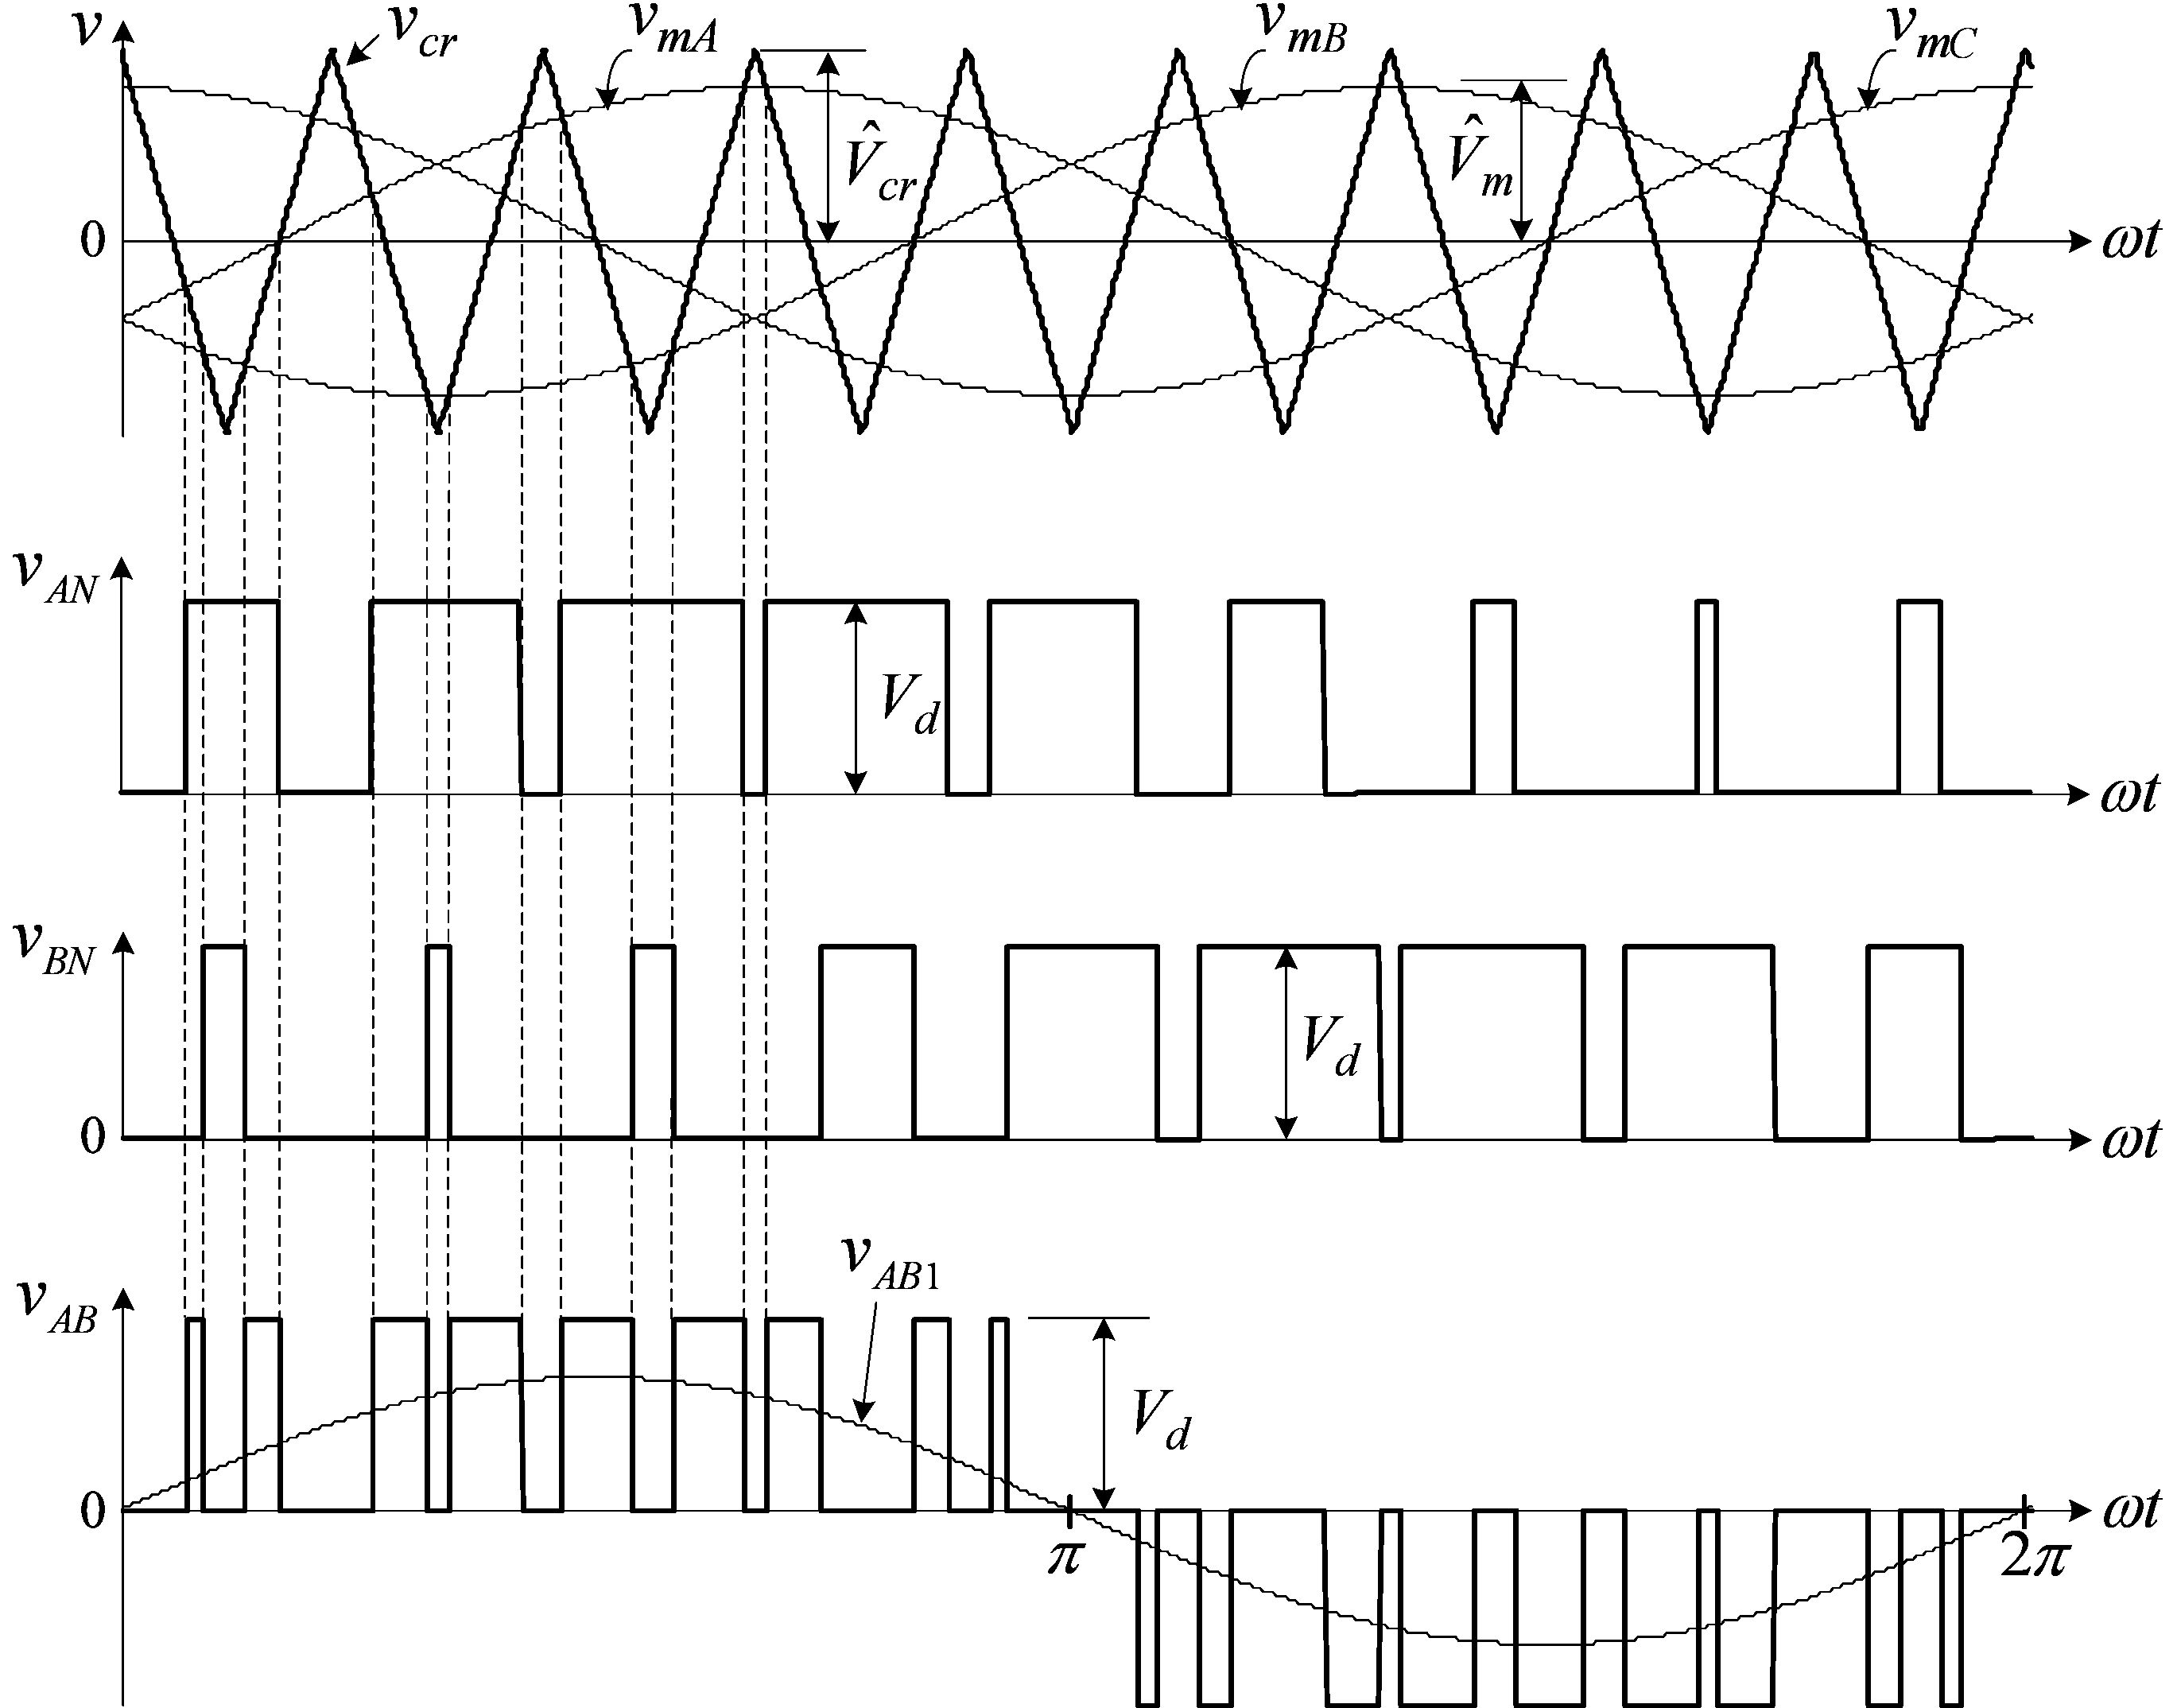
\includegraphics[width=0.5\textheight]{graficos/img62.jpg}
	\caption{Figure 6.2-1 Sinusoidal pulse-width modulation (SPWM).}
\end{figure}
\FloatBarrier

where $V_m$ and $V_{cr}$ are the peak values of the modulating and carrier waves, respectively. The amplitude modulation index $m_a$ is usually adjusted by varying $V_m$ while keeping $V_{cr}$ fixed. The \textbf{frequency modulation index} is defined by
\[
	m_f = \frac{f_{cr}}{f_m}
\]
where $f_m$ and $f_{cr}$ are the frequencies of the modulating and carrier waves, respectively.

The operation of switches $S_1$ to $S_6$ is determined by comparing the modulating waves with the carrier wave. When $V_{m_a} > V_{cr}$, the upper switch $S_1$ in inverter leg A is turned on. The lower switch $S_4$ operates in a complementary manner and thus is switched off. The resultant \textit{inverter terminal voltage} $V_{AN}$, which is the voltage at the phase A terminal with respect to the negative dc bus $N$, is equal to the dc voltage $V_d$. When $V_{m_a} < V_{cr}$, $S_1$ is on and $S_4$ is off, leading to $V_{AN} = 0$ as shown in Fig. 6.2-1. Since the waveform of $V_{AN}$ has only two levels, $V_d$ and 0, the inverter is known as a \textit{two-level inverter}. It should be noted that to avoid possible short circuit during switching transients of the upper and lower devices in an inverter leg, a \textit{blanking time} should be implemented, during which both switches are turned off.

The inverter line-to-line voltage $V_{AB}$ can be determined by $V_{AB} = V_{AN} - V_{BN}$. The waveform of its fundamental-frequency component $V_{AB1}$ is also given in the figure. The magnitude and frequency of $V_{AB1}$ can be independently controlled by $m_a$ and $f_m$, respectively.

The \textbf{switching frequency} of the active switches in the two-level inverter can be found from $f_{sw} = f_{cr} - f_m \times m_f$. For instance, $V_{AN}$ in Fig. 6.2-1 contains nine pulses per cycle of the fundamental frequency. Each pulse is produced by turning $S_1$ on and off once. With the fundamental frequency of 60 Hz, the resultant switching frequency for $S_1$ is $f_{sw} = 60 \times 9 = 540$ Hz, which is also the carrier frequency $f_{cr}$. It is worth noting that the device switching frequency may not always be equal to the carrier frequency in multilevel inverters. This issue will be addressed in the later chapters.

When the carrier wave is synchronized with the modulating wave ($m_f$ is an integer), the modulation scheme is known as \textbf{synchronous PWM}, in contrast to \textbf{asynchronous PWM} whose carrier frequency $f_{cr}$ is usually fixed and independent of $f_m$. The asynchronous PWM features a fixed switching frequency and easy implementation with analog circuits. However, it may generate noncharacteristic harmonics, whose frequency is not a multiple of the fundamental frequency. The synchronous PWM scheme is more suitable for implementation with a digital processor.

\subsubsection{Harmonic Content}
Figure 6.2-2 shows a set of simulated waveforms for the two-level inverter, where $V_{AB}$ is the inverter line-to-line voltage, $V_{A0}$ is the load phase voltage and $i_4$ is the load current. The inverter operates under the condition of $m_a = 0.8$, $m_f = 15$, $f_m = 60$ Hz, and $f_{sw} = 900$ Hz with a rated three-phase inductive load. The load power factor is 0.9 per phase. We can observe the following:

\begin{itemize}
	\item All the harmonics in $V_{AB}$ with the order lower than $(m_f - 2)$ are eliminated.
	\item The harmonics are centered around $m_f$ and its multiples such as $2m_f$ and $3m_f$.
\end{itemize}

The above statements are valid for $m_f \geq 9$ provided that $m_f$ is a multiple of 3 [1]. The waveform of the load current $i_4$ is close to sinusoidal with a THD of 7.73\%. The low amount of harmonic distortion is due to the elimination of low-order harmonics by the modulation scheme and the filtering effect of the load inductance.

Figure 6.2-3 shows the harmonic content of the inverter line-to-line voltage $V_{AB}$ normalized to its dc voltage $V_d$ as a function of $m_a$, where $V_{ABn}$ is the nth-order harmonic voltage (rms). The fundamental-frequency component $V_{AB1}$ increases linearly with $m_a$, whose maximum value can be found from
\[
	V_{AB1,\text{max}} = 0.612 V_d \quad \text{for } m_a = 1
\]
The THD curve for $V_{AB}$ is also given in the figure.

\begin{figure}[h]
	\centering
	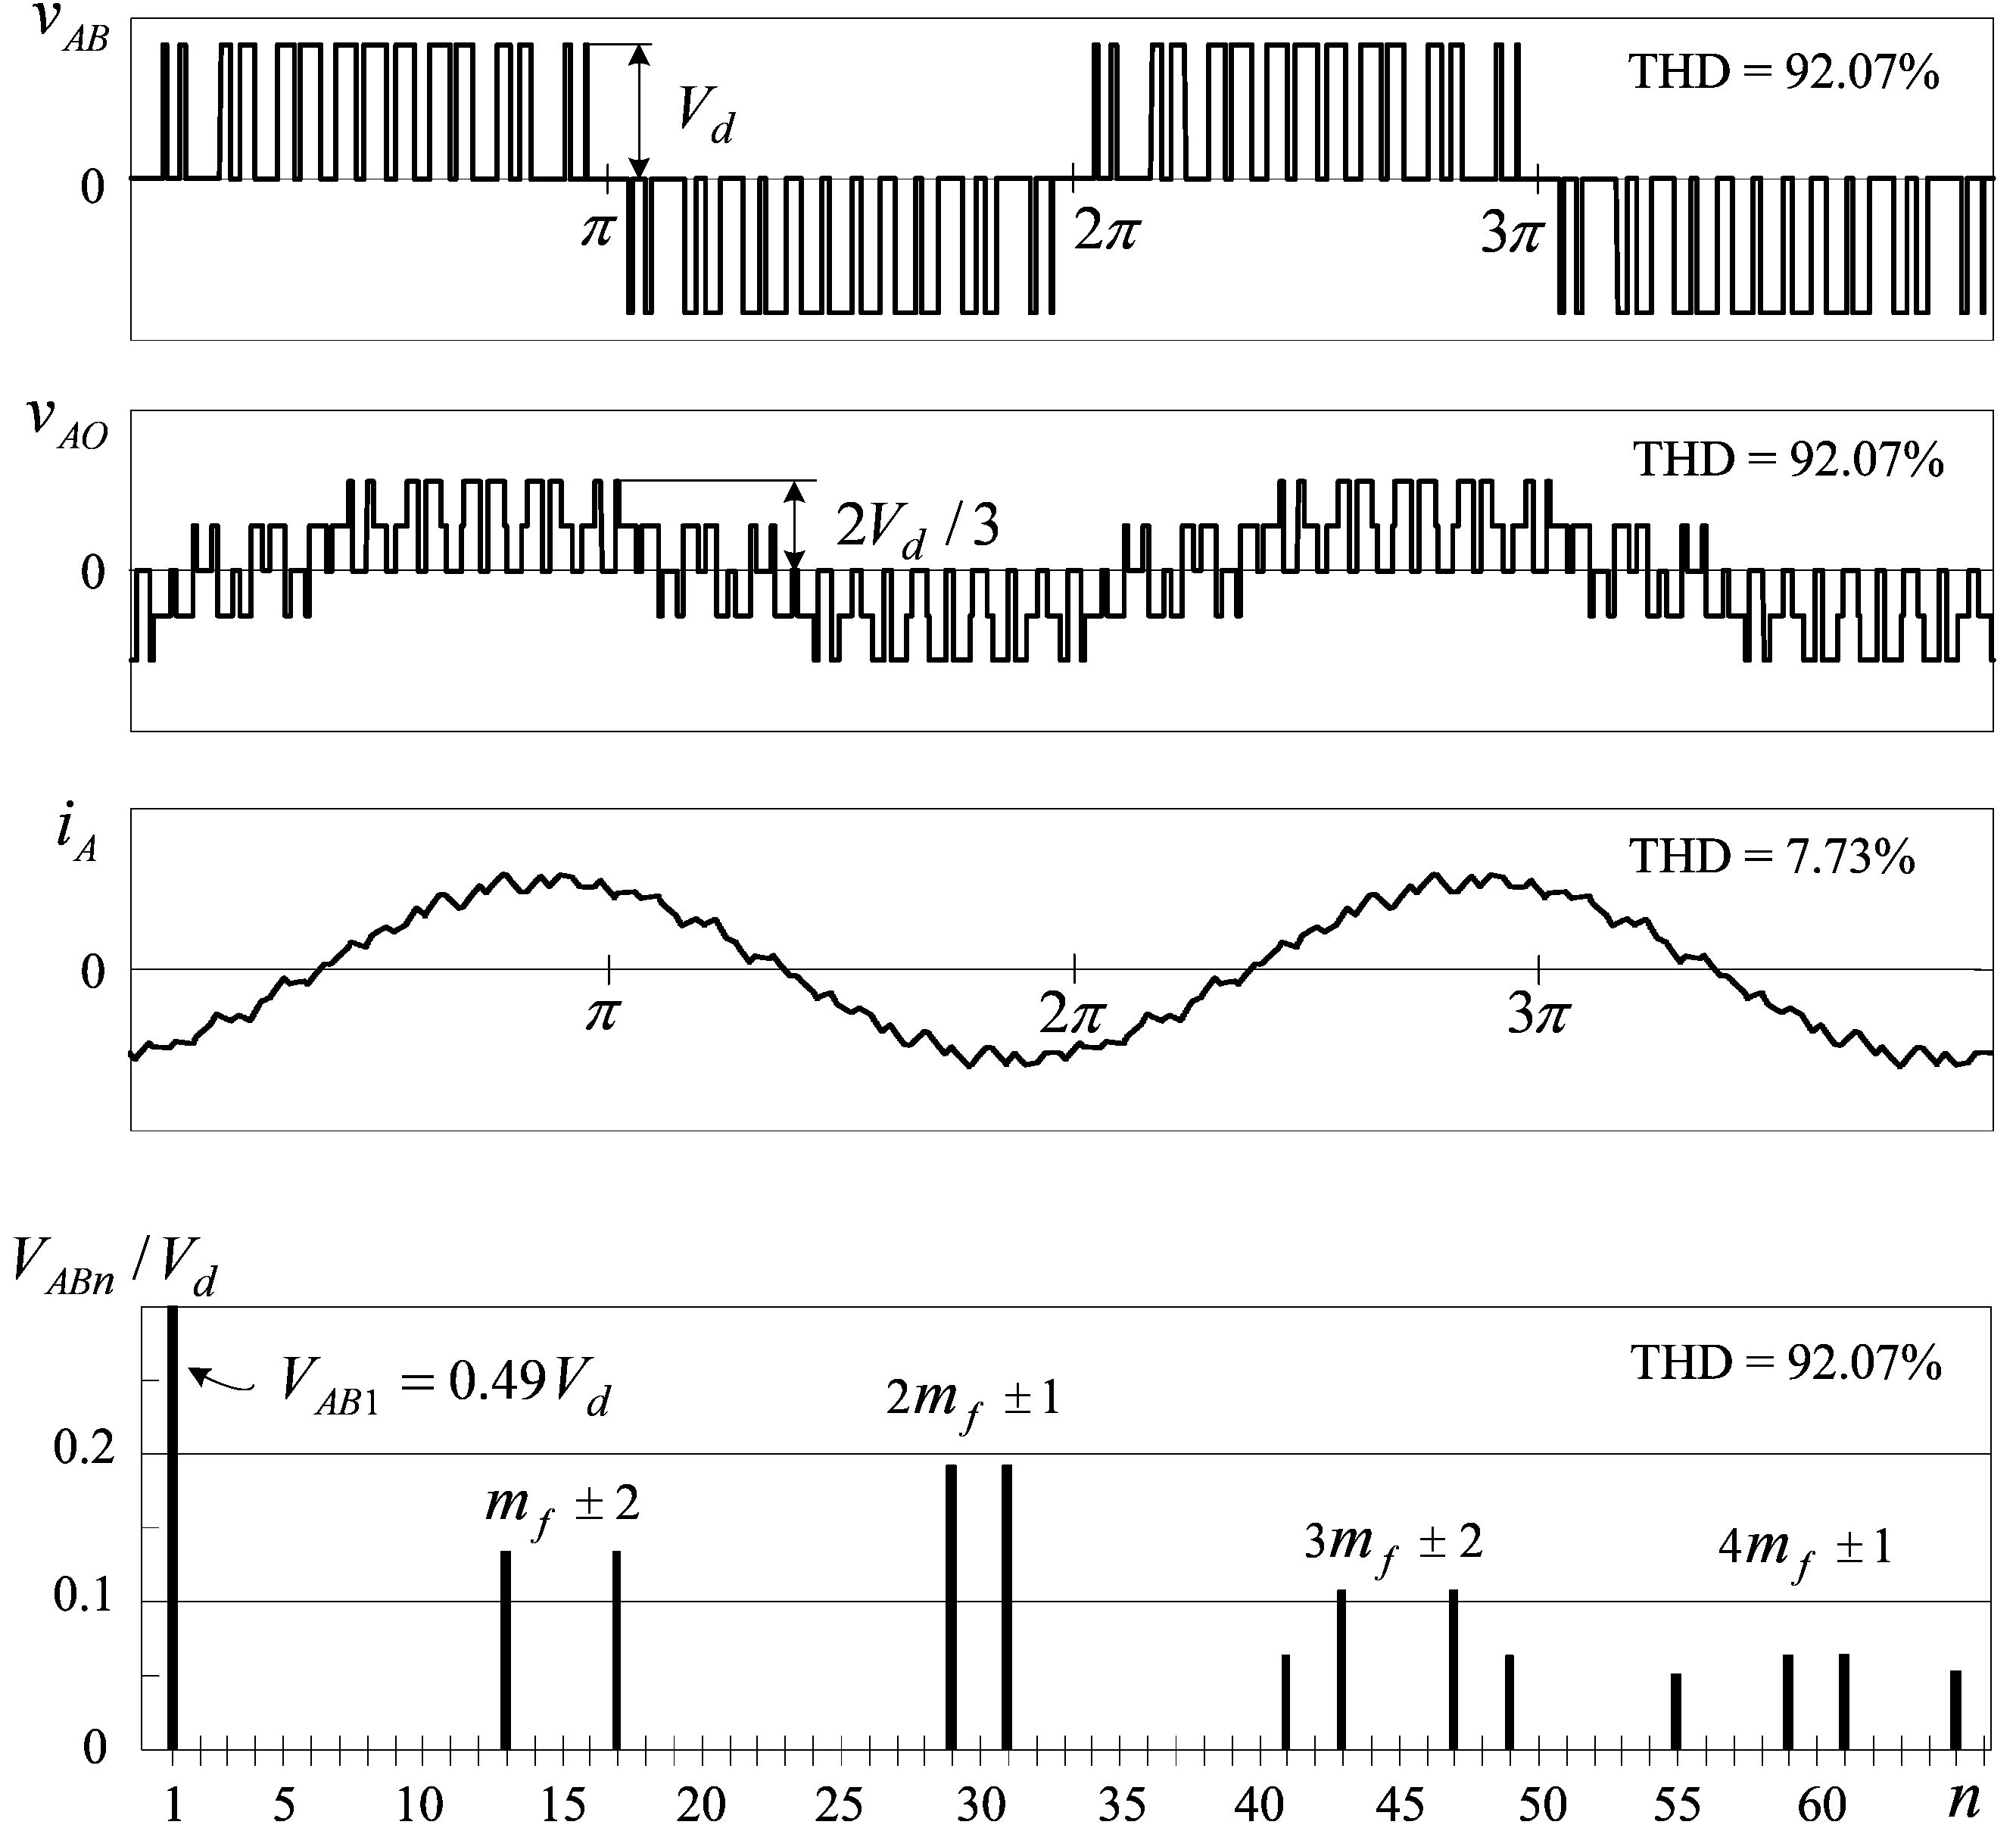
\includegraphics[width=0.9\textwidth]{graficos/img71.jpg}
	\caption{Figure 6.2-3 Simulated waveforms for the two-level inverter operating at $m_a = 0.8$, $m_f = 15$, $f_m = 60$ Hz, and $f_{sw} = 900$ Hz.}
\end{figure}
\FloatBarrier

\begin{figure}[h]
	\centering
	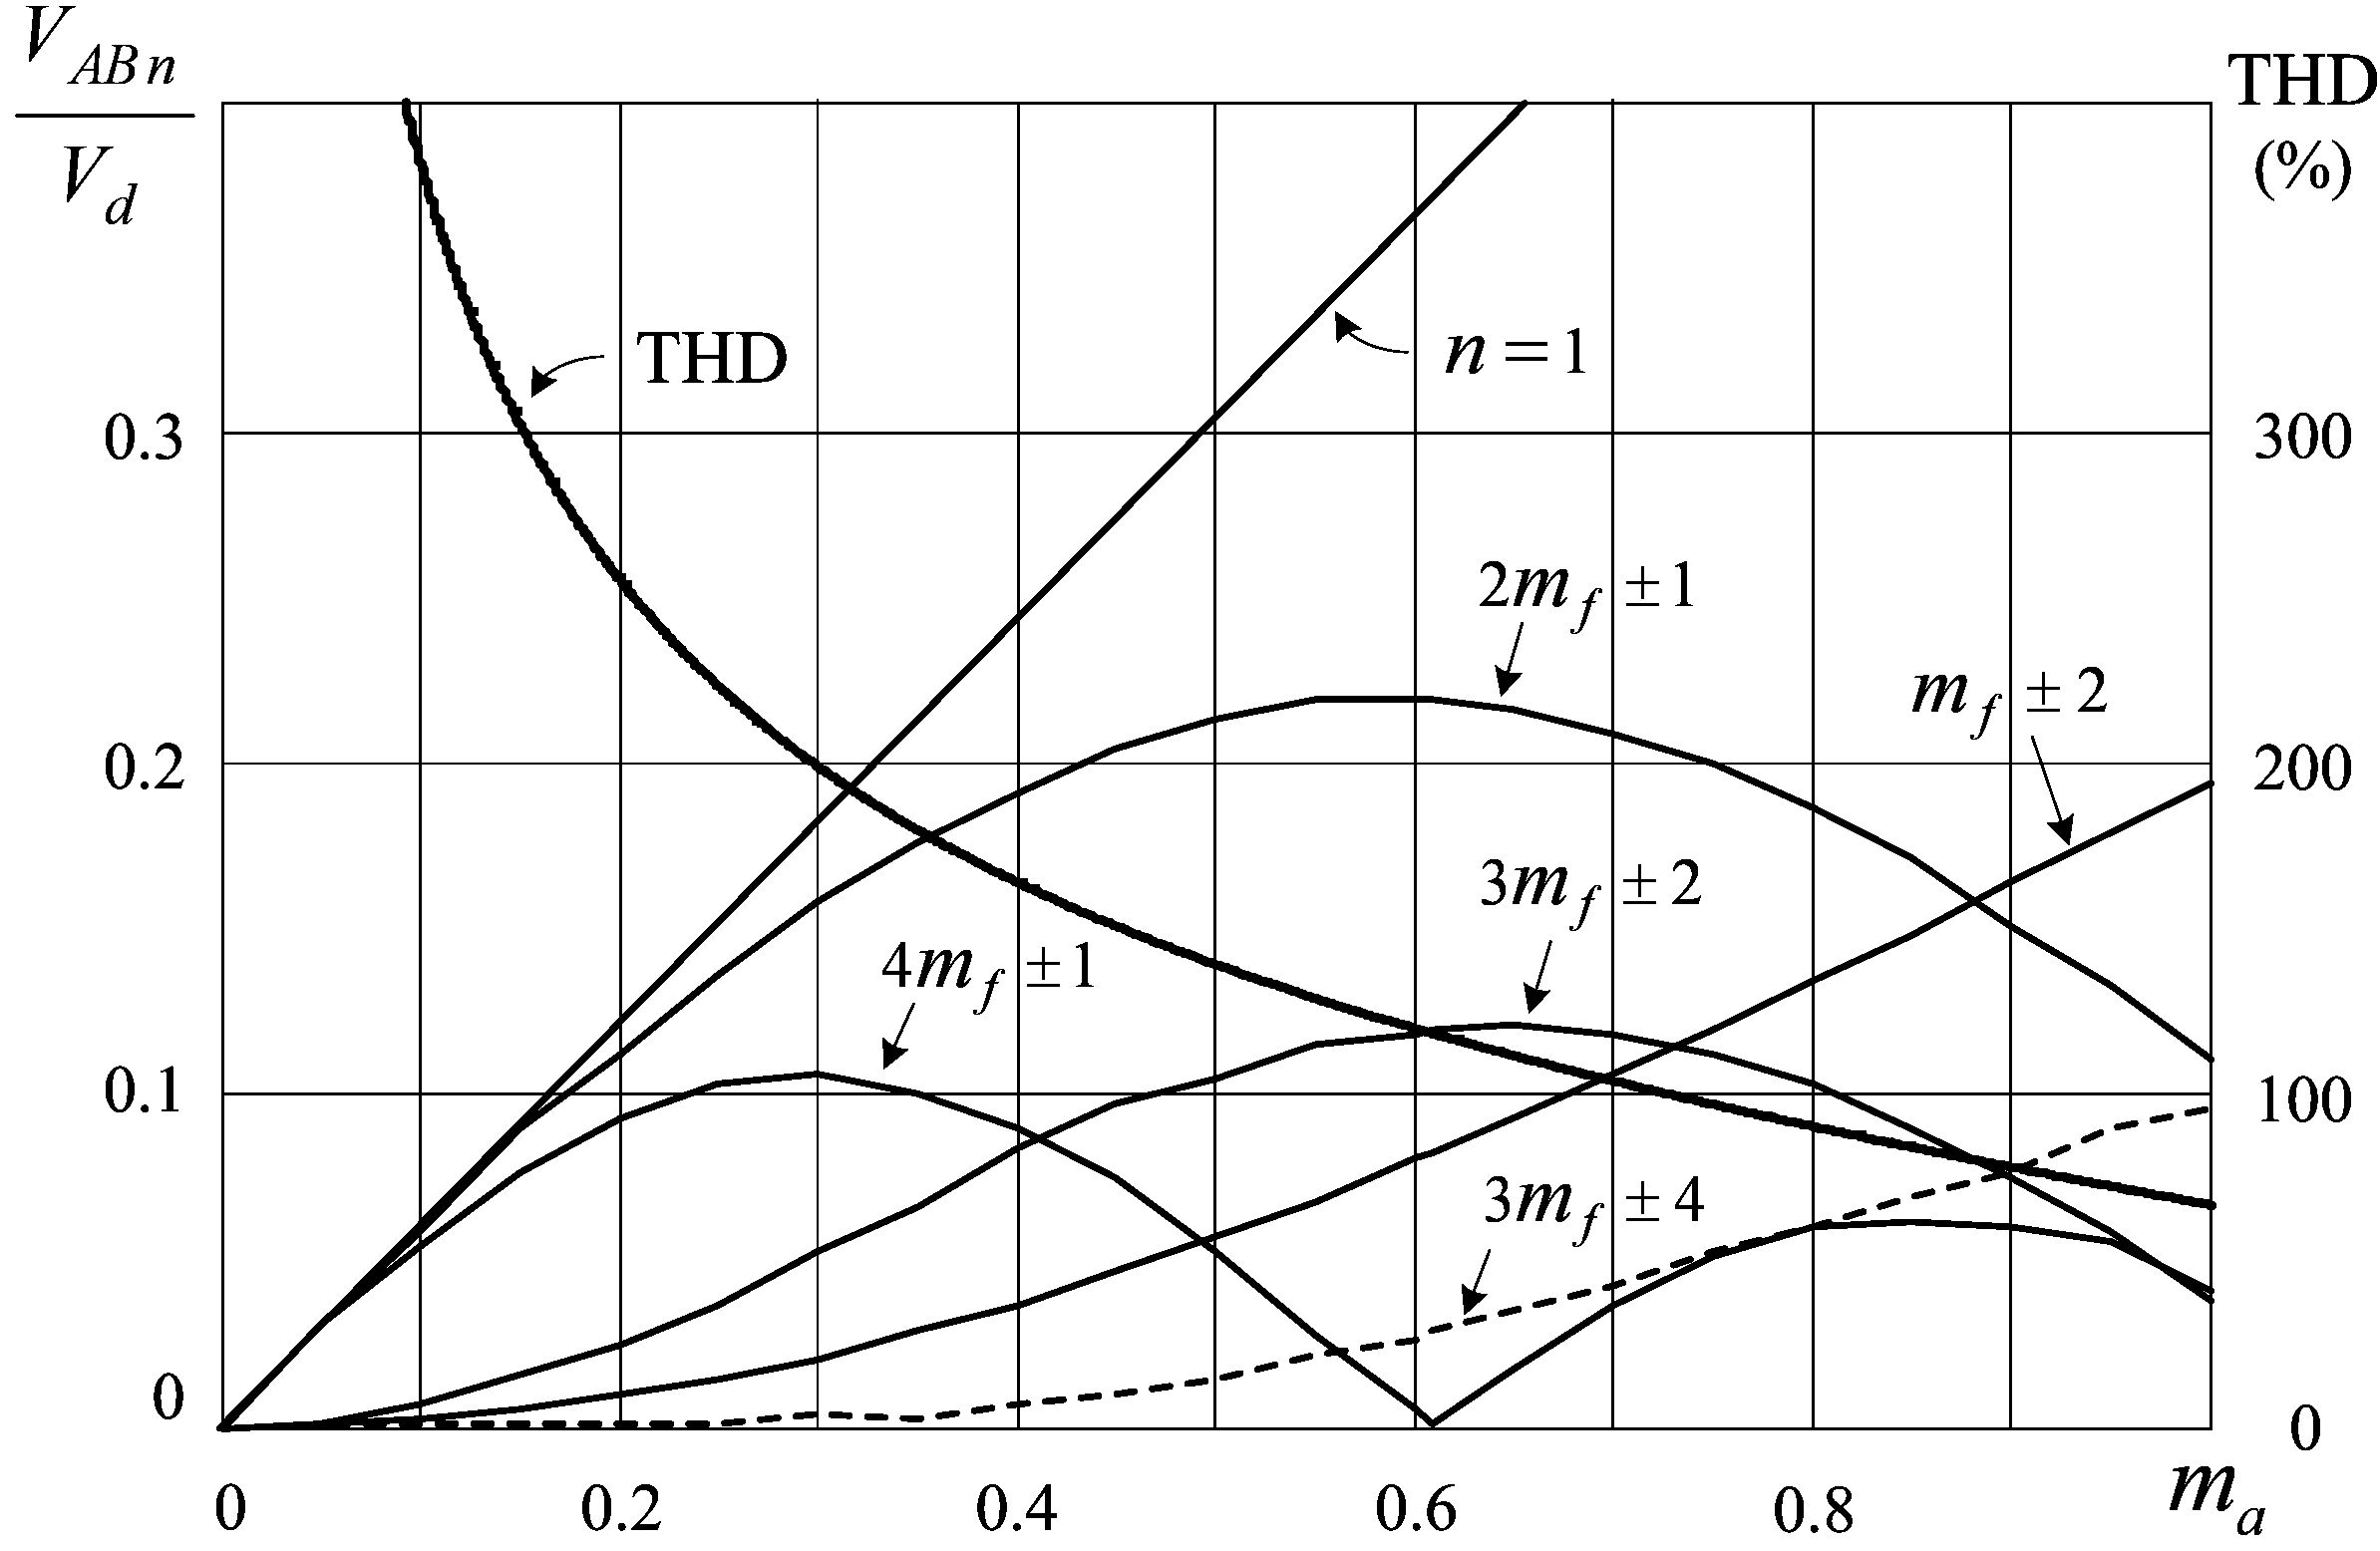
\includegraphics[width=0.8\textwidth]{graficos/img80.jpg}
	\caption{Figure 6.2-3 Harmonic content of $V_{AB}$ in Fig. 6.2-2.}
\end{figure}
\FloatBarrier


\subsection{Overmodulation}
Overmodulation occurs when the amplitude modulation index $m_a$ is greater than unity. Figure 6.2-4 shows such a case with $m_a = 2$. The overmodulation causes a reduction in number of pulses in the line-to-line voltage waveform, leading to the emergence of low-order harmonics such as the 5th and 11th. However, the fundamental voltage $V_{AB1}$ is boosted to 0.744$V_d$, which represents a 22\% increase in comparison with 0.612$V_d$ at $m_a = 1$. With $m_a$ further increased to 3.24, $V_{AB}$ becomes a square wave, whose fundamental voltage is $V_{AB1} = 0.78V_d$, which is the highest possible value produced by the two-level VSI. The overmodulation is seldom used in practice due to the difficulties to filter out the low-order harmonics and the nonlinear relationship between $V_{AB1}$ and $m_a$.

\subsubsection{Third Harmonic Injection PWM}
The inverter fundamental voltage $V_{AB1}$ can also be increased by adding a third harmonic component to the three-phase sinusoidal modulating wave without causing overmodulation. This modulation technique is known as \textit{third harmonic injection PWM}.

Figure 6.2-5 illustrates the principle of this PWM scheme, where the modulating wave $v_{m4}$ is composed of a fundamental component $v_{m1}$ and a third harmonic component $v_{m3}$, making $v_{m4}$ somewhat flattened on the top. As a result, the peak fundamental component $v_{m1}$ can be higher than the peak triangular carrier wave $v_{cr}$, which boosts the fundamental voltage $V_{AB1}$. In the meantime the peak modulating wave $v_{m4}$ can be kept lower than $v_{cr}$, avoiding the problems caused by overmodulation. The maximum amount of $V_{AB1}$ that can be increased by this scheme is 15.5\% [2, 3].

\begin{figure}[h]
	\centering
	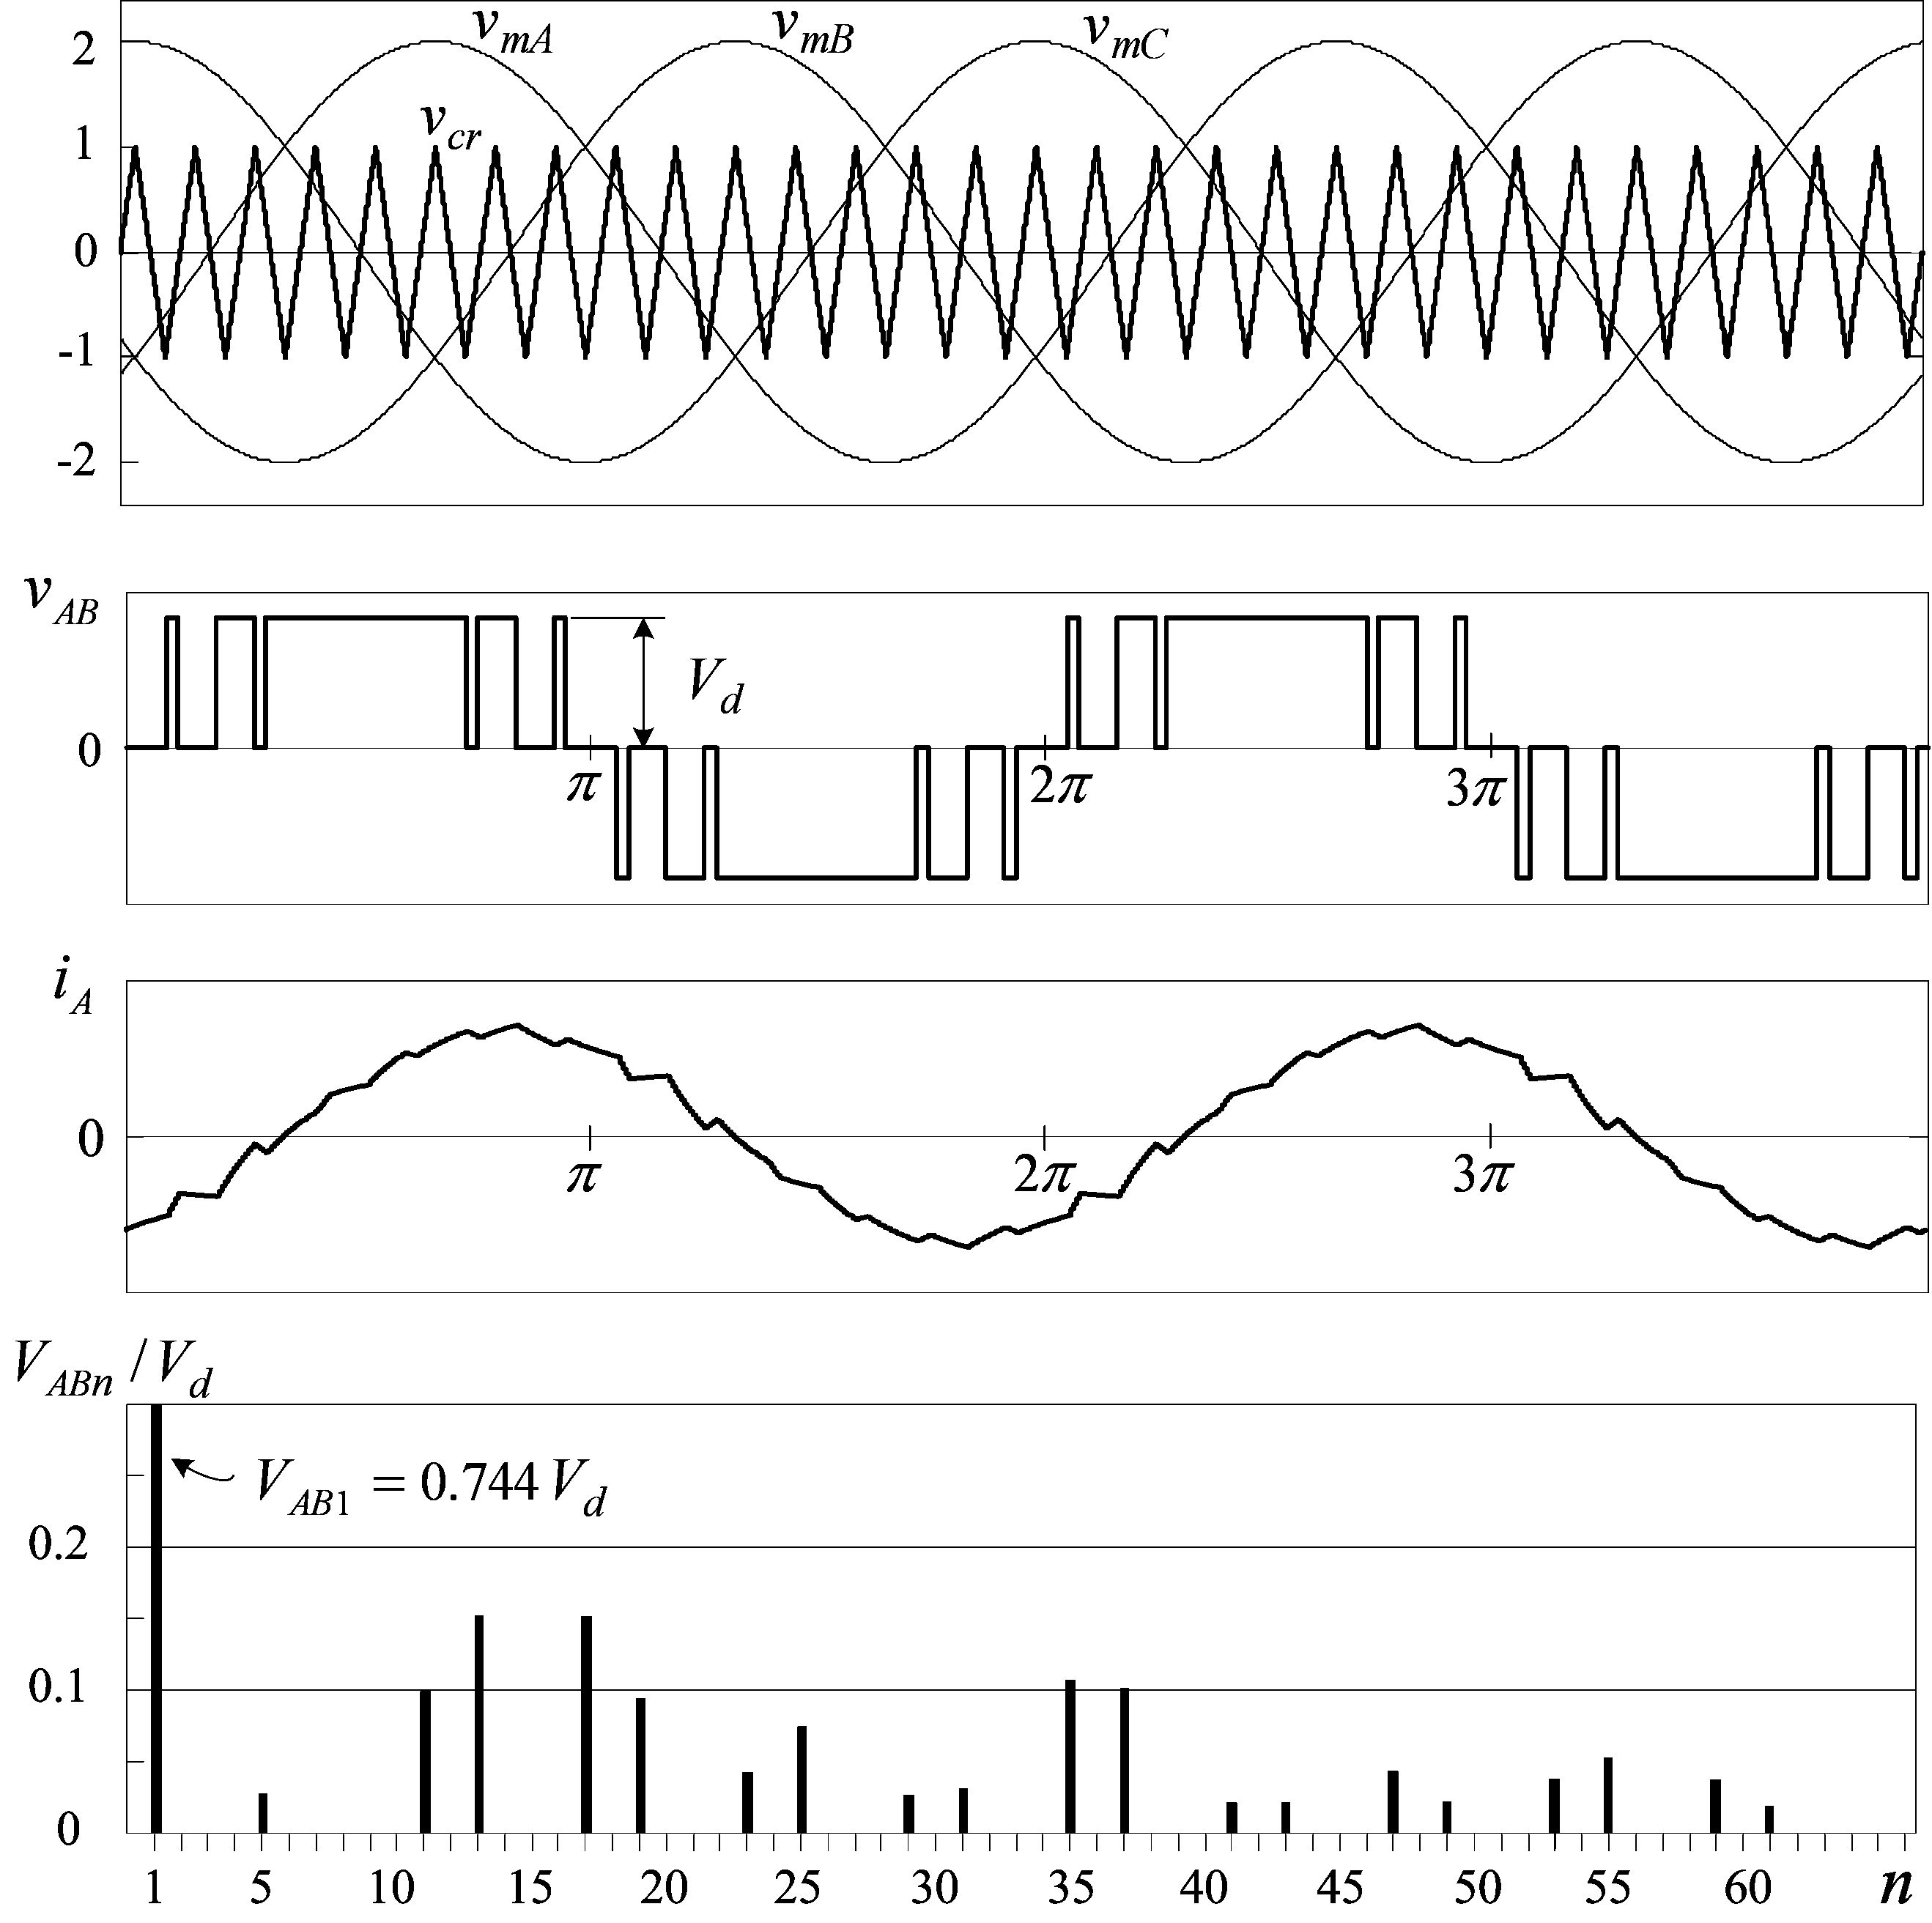
\includegraphics[width=0.5\textheight]{graficos/img85.jpg}
	\caption{Figure 6.2-4 Overmodulation ($m_a = 2.0$, $m_f = 15$, and $f_m = 60$ Hz).}
\end{figure}
\FloatBarrier

\begin{figure}[h]
	\centering
	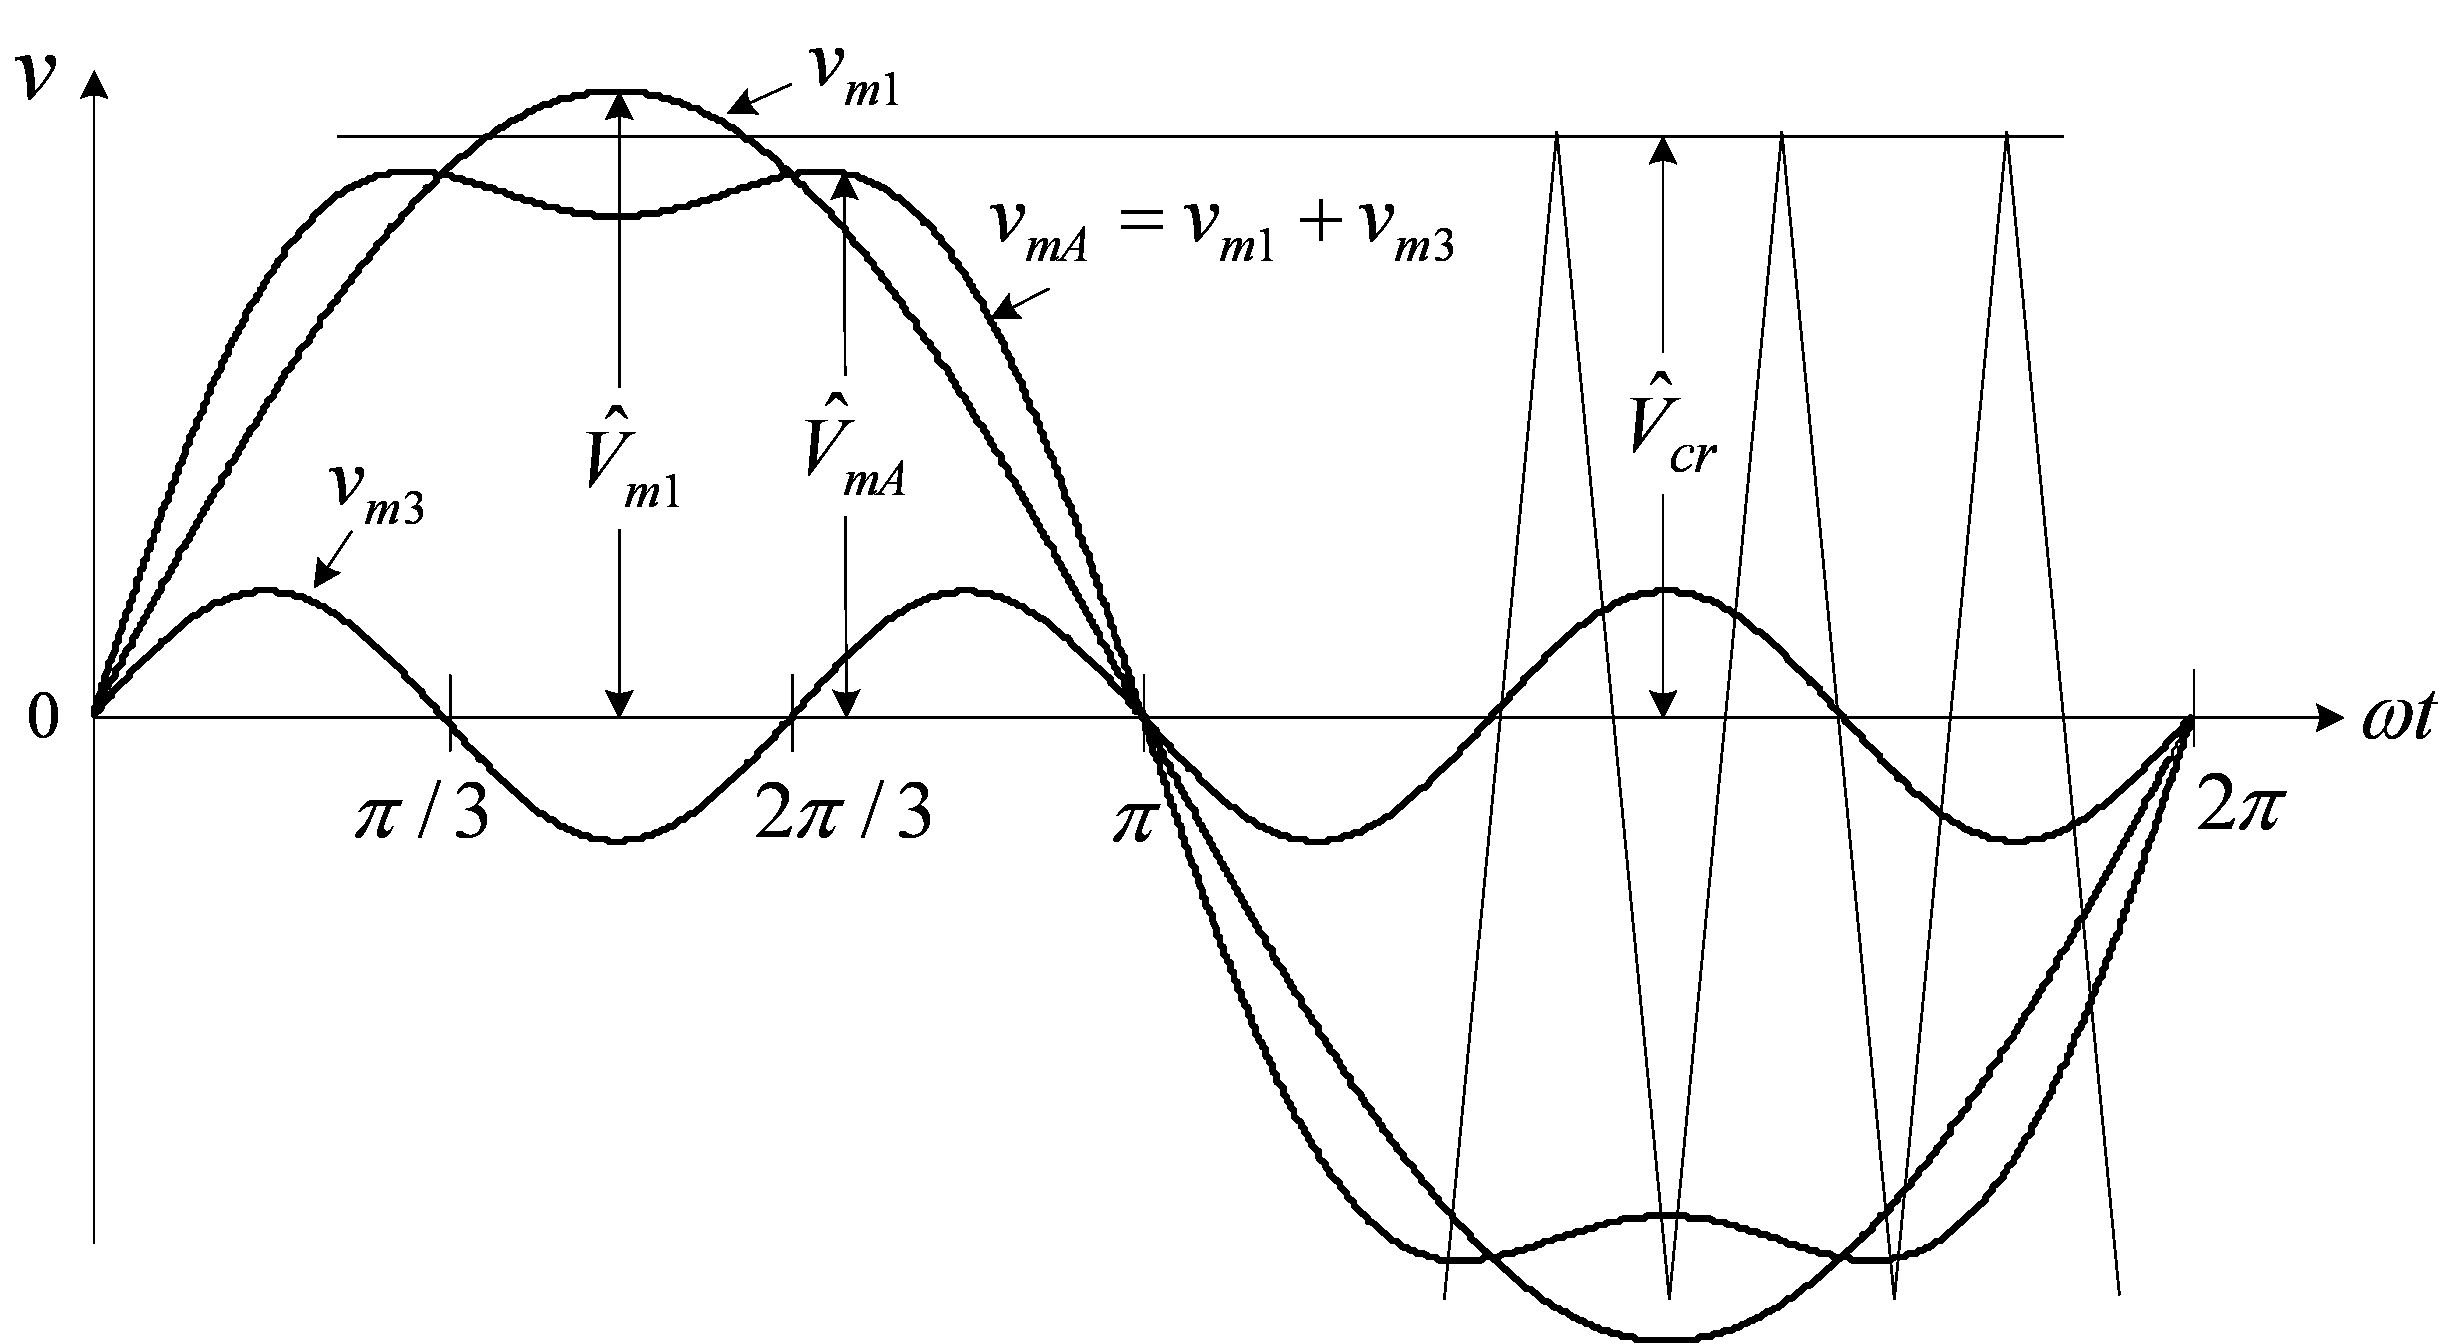
\includegraphics[width=0.5\textheight]{graficos/img86.jpg}
	\caption{Figure 6.2-5 Modulating wave $v_{m4}$ with third harmonic injection.}
\end{figure}
\FloatBarrier

The injected third harmonic component $v_{m3}$ will not increase the harmonic distortion for $V_{AB}$. Although it appears in each of the inverter terminal voltages $V_{AN}$, $V_{BN}$ and $V_{CN}$, the third-order harmonic voltage does not exist in the line-to-line voltage $V_{AB}$. This is because the line-to-line voltage is given by $V_{AB} = V_{AN} - V_{BN}$, where the third-order harmonics in $V_{AN}$ and $V_{BN}$ are of zero sequence with the same magnitude and phase displacement and thus cancel each other.

\section{Space Vector Modulation}

Space vector modulation (SVM) is one of the preferred real-time modulation techniques and is widely used for digital control of voltage source inverters [3, 4]. This section presents the principle and implementation of the space vector modulation for the two-level inverter.

\subsection{Switching States}
The operating status of the switches in the two-level inverter in Fig. 6.1-1 can be represented by switching states. As indicated in Table 6.3-1, switching state `P' denotes that the upper switch in an inverter leg is on and the inverter terminal voltage ($V_{AN}$, $V_{BN}$, or $V_{CN}$) is positive ($+V_d$) while `O' indicates that the inverter terminal voltage is zero due to the conduction of the lower switch.

There are eight possible combinations of switching states in the two-level inverter as listed in Table 6.3-2. The switching state [POO], for example, corresponds to the conduction of $S_1$, $S_6$, and $S_2$ in the inverter legs A, B, and C, respectively. Among the eight switching states, [PPP] and [OOO] are zero states and the others are active states.

\subsection{Space Vectors}
The active and zero switching states can be represented by active and zero space vectors, respectively. A typical space vector diagram for the two-level inverter is shown in Fig. 6.3-1, where the six active vectors $V_1$ to $V_6$ form a regular hexagon with six equal sectors (I to VI). The zero vector $V_0$ lies on the center of the hexagon.

\begin{table}[h]
    \centering
    \caption{Table 6.3-1 Definition of Switching States}
    \begin{tabular}{c c c c c c c c c c}
        \hline
        \textbf{Switching} & & \textbf{Leg A} & & & \textbf{Leg B} & & & \textbf{Leg C} & \\
        \hline
        \textbf{State} & $S_1$ & $S_4$ & $V_{AN}$ & $S_3$ & $S_6$ & $V_{BN}$ & $S_5$ & $S_2$ & $V_{CN}$ \\
        \hline
        P & On & Off & $V_d$ &  On & Off & $V_d$ & On & Off & $V_d$ \\
        O & Off & On & 0 & Off & On & 0 & Off & On & 0 \\
        \hline
    \end{tabular}
    \label{table:switching_states}
\end{table}
\FloatBarrier

\begin{table}[h]
    \centering
    \caption{Table 6.3-2 Space Vectors, Switching States, and On-State Switches}
    \begin{tabular}{c c c c c}
    \hline
    & & \textbf{Switching State} & & \textbf{Vector} \\
        \textbf{Space Vector}  & & \textbf{(Three Phases)} & \textbf{On-State Switch} & \textbf{Definition} \\
    \hline
    Zero Vector & $\mathbf{V}_7$ & [PPP] & $S_1, S_3, S_5$ & $\mathbf{V}_0 = 0$ \\
                & $\mathbf{V}_0$ & [OOO] & $S_4, S_6, S_2$ & $\mathbf{V}_0 = 0$ \\ [1em]
    Active Vector & $\mathbf{V}_1$ & [POO] & $S_1, S_6, S_2$ & $\mathbf{V}_1 = \frac{2}{3} V_{dc}e^{j0}$ \\[0.5em]
    & $\mathbf{V}_2$ & [PPO] & $S_1, S_3, S_2$ & $\mathbf{V}_2 = \frac{2}{3} V_{dc}e^{j\frac{\pi}{3}}$ \\[0.5em]
    & $\mathbf{V}_3$ & [OPO] & $S_4, S_3, S_2$ & $\mathbf{V}_3 = \frac{2}{3} V_{dc}e^{j\frac{2\pi}{3}}$ \\[0.5em]
    & $\mathbf{V}_4$ & [OPP] & $S_4, S_3, S_5$ & $\mathbf{V}_4 = \frac{2}{3} V_{dc}e^{j\pi}$ \\[0.5em]
    & $\mathbf{V}_5$ & [OOP] & $S_4, S_6, S_5$ & $\mathbf{V}_5 = \frac{2}{3} V_{dc}e^{j\frac{4\pi}{3}}$ \\[0.5em]
    & $\mathbf{V}_6$ & [POP] & $S_1, S_6, S_5$ & $\mathbf{V}_6 = \frac{2}{3} V_{dc}e^{j\frac{5\pi}{3}}$ \\[0.5em]
    \hline
    \end{tabular}
    \label{table:space_vectors}
\end{table}
\FloatBarrier
    
To derive the relationship between the space vectors and switching states, refer to the two-level inverter in Fig. 6.1-1. Assuming that the operation of the inverter is three-phase balanced, we have
\[
V_{AO}(t) + V_{BO}(t) + V_{CO}(t) = 0
\]
where $V_{AO}$, $V_{BO}$, and $V_{CO}$ are the instantaneous load phase voltages. From mathematical point of view, one of the phase voltages is redundant since given any two phase
    
\begin{figure}[h]
    \centering
    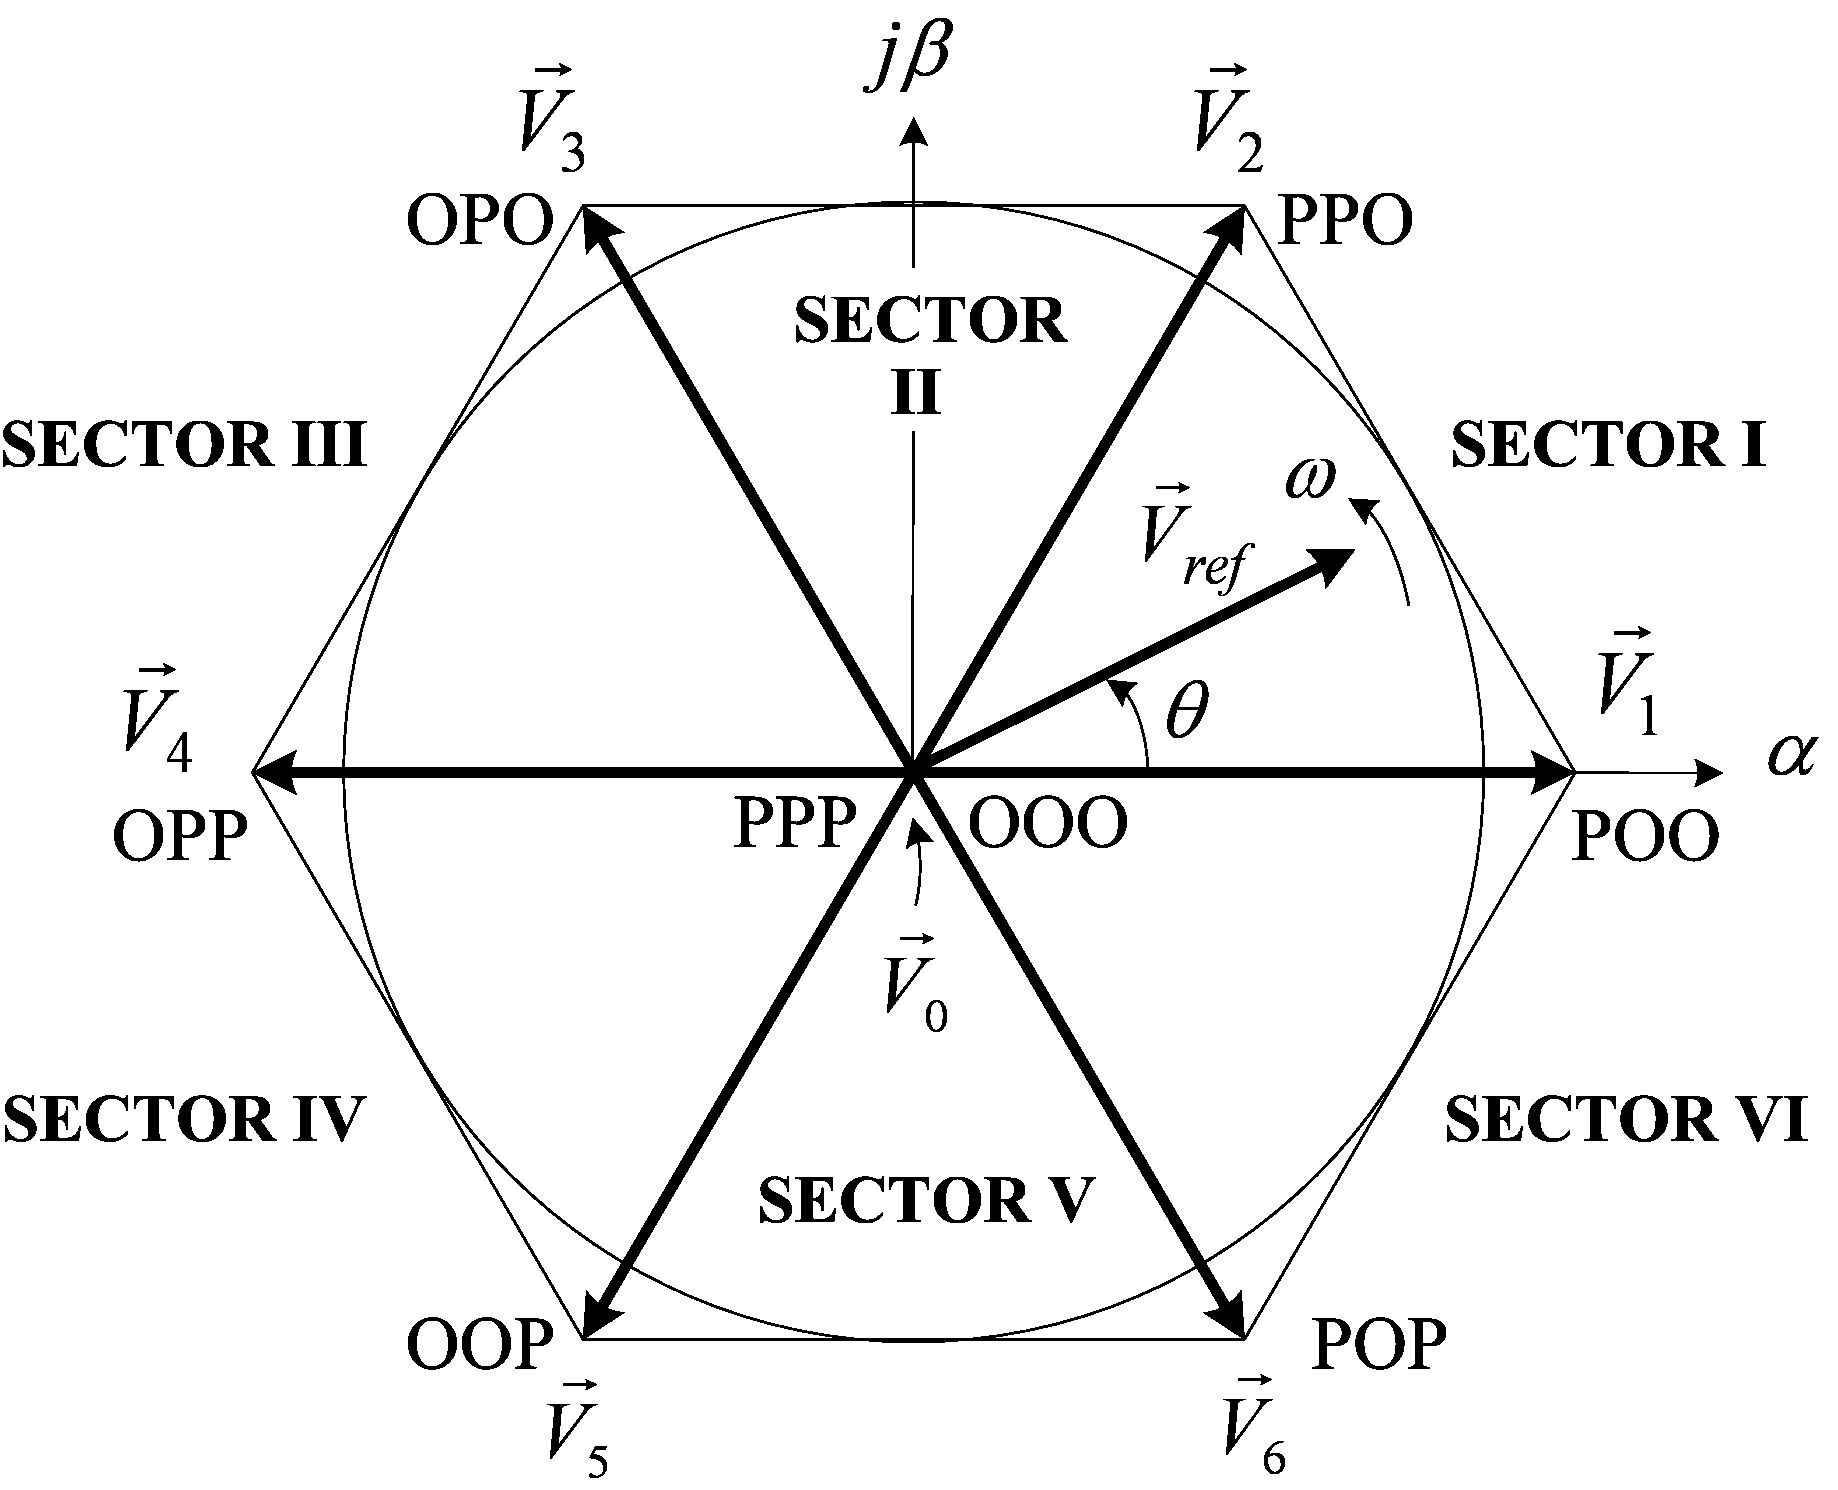
\includegraphics[width=0.6\textwidth]{graficos/img99.jpg}
    \caption{Figure 6.3-1 Space vector diagram for the two-level inverter.}
    \label{fig:space_vector_diagram}
\end{figure}
\FloatBarrier

voltages, the third one can be readily calculated. Therefore, it is possible to transform the three-phase variables to equivalent two-phase variables [5]:
\[
\begin{bmatrix}
v_{\alpha}(t) \\
v_{\beta}(t)
\end{bmatrix}
= \frac{2}{3}
\begin{bmatrix}
1 & -\frac{1}{2} & -\frac{1}{2} \\
0 & \frac{\sqrt{3}}{2} & -\frac{\sqrt{3}}{2}
\end{bmatrix}
\begin{bmatrix}
V_{AO}(t) \\
V_{BO}(t) \\
V_{CO}(t)
\end{bmatrix}
\]

The coefficient $\frac{2}{3}$ is somewhat arbitrarily chosen. The commonly used value is $\frac{2}{3}$ or $\frac{\sqrt{2}}{3}$. The main advantage of using $\frac{2}{3}$ is that the magnitude of the two-phase voltages will be equal to that of the three-phase voltages after the transformation. A space vector can be generally expressed in terms of the two-phase voltages in the $\alpha$-$\beta$ plane:

\[
\mathbf{\hat{V}}(t) = v_{\alpha}(t) + jv_{\beta}(t)
\]

Substituting (6.3-2) into (6.3-3), we have:

\[
\mathbf{\hat{V}}(t) = \frac{2}{3} [V_{AO}(t)e^{j0} + V_{BO}(t)e^{j\frac{2\pi}{3}} + V_{CO}(t)e^{j\frac{4\pi}{3}}]
\]

where $e^{jx} = \cos x + j\sin x$ and $x = 0, \frac{2\pi}{3}$ or $\frac{4\pi}{3}$. For active switching state [POO], the generated load phase voltages are:

\[
V_{AO}(t) = \frac{2}{3} V_d, \quad V_{BO}(t) = -\frac{1}{3} V_d, \quad V_{CO}(t) = -\frac{1}{3} V_d
\]

The corresponding space vector, denoted as $\mathbf{V}_1$, can be obtained by substituting (6.3-5) into (6.3-4):

\[
\mathbf{V}_1 = \frac{2}{3} V_d e^{j0}
\]

Following the same procedure, all six active vectors can be derived:

\[
\mathbf{V}_k = \frac{2}{3} V_d e^{j\left(k-1\right) \frac{\pi}{3}}, \quad k = 1, 2, \ldots, 6
\]

The zero vector $\mathbf{V}_0$ has two switching states [PPP] and [OOO], one of which seems redundant. As will be seen later, the redundant switching state can be utilized to minimize the switching frequency of the inverter or perform other useful functions. The relationship between the space vectors and their corresponding switching states is given in Table 6.3-2.

Note that the zero and active vectors do not move in space, and thus they are referred to as stationary vectors. On the contrary, the reference vector $\mathbf{V}_{ref}$ in Fig. 6.3-1 rotates in space at an angular velocity.

\[
\omega = 2\pi f_1 \tag{6.3-8}
\]
where \( f_1 \) is the fundamental frequency of the inverter output voltage. The angular displacement between \( \mathbf{V}_{\text{ref}} \) and the \(\alpha\)-axis of the \(\alpha\)-\(\beta\) plane can be obtained by
\[
\theta(t) = \int_0^t \omega(t') \, dt' + \theta(0) \tag{6.3-9}
\]

For a given magnitude (length) and position, \( \mathbf{V}_{\text{ref}} \) can be synthesized by three near-stationary vectors, based on which the switching states of the inverter can be selected and gate signals for the active switches can be generated. When \( \mathbf{V}_{\text{ref}} \) passes through sectors one by one, different sets of switches will be turned on or off. As a result, when \( \mathbf{V}_{\text{ref}} \) rotates one revolution in space, the inverter output voltage varies one cycle over time. The inverter output frequency corresponds to the rotating speed of \( \mathbf{V}_{\text{ref}} \), while its output voltage can be adjusted by the magnitude of \( \mathbf{V}_{\text{ref}} \).

\section*{6.3.3 Dwell Time Calculation}

As mentioned earlier, the reference $\mathbf{V}_{\text{ref}}$ can be synthesized by three stationary vectors. The dwell time for the stationary vectors essentially represents the duty-cycle time (on-state or off-state time) of the chosen switches during a sampling period $T_s$ of the modulation scheme. The dwell time calculation is based on ``volt-second balancing'' principle, that is, the product of the reference voltage $\mathbf{V}_{\text{ref}}$ and sampling period $T_s$ equals the sum of the voltage multiplied by the time interval of chosen space vectors.

Assuming that the sampling period $T_s$ is sufficiently small, the reference vector $\mathbf{V}_{\text{ref}}$ can be considered constant during $T_s$. Under this assumption, $\mathbf{V}_{\text{ref}}$ can be approximated by two adjacent active vectors and one zero vector. For example, when $\mathbf{V}_{\text{ref}}$ is in Sector I as shown in Figure 6.3-2, it can be synthesized by $\mathbf{V}_1$, $\mathbf{V}_2$, and $\mathbf{V}_0$.

\begin{figure}[h]
    \centering
    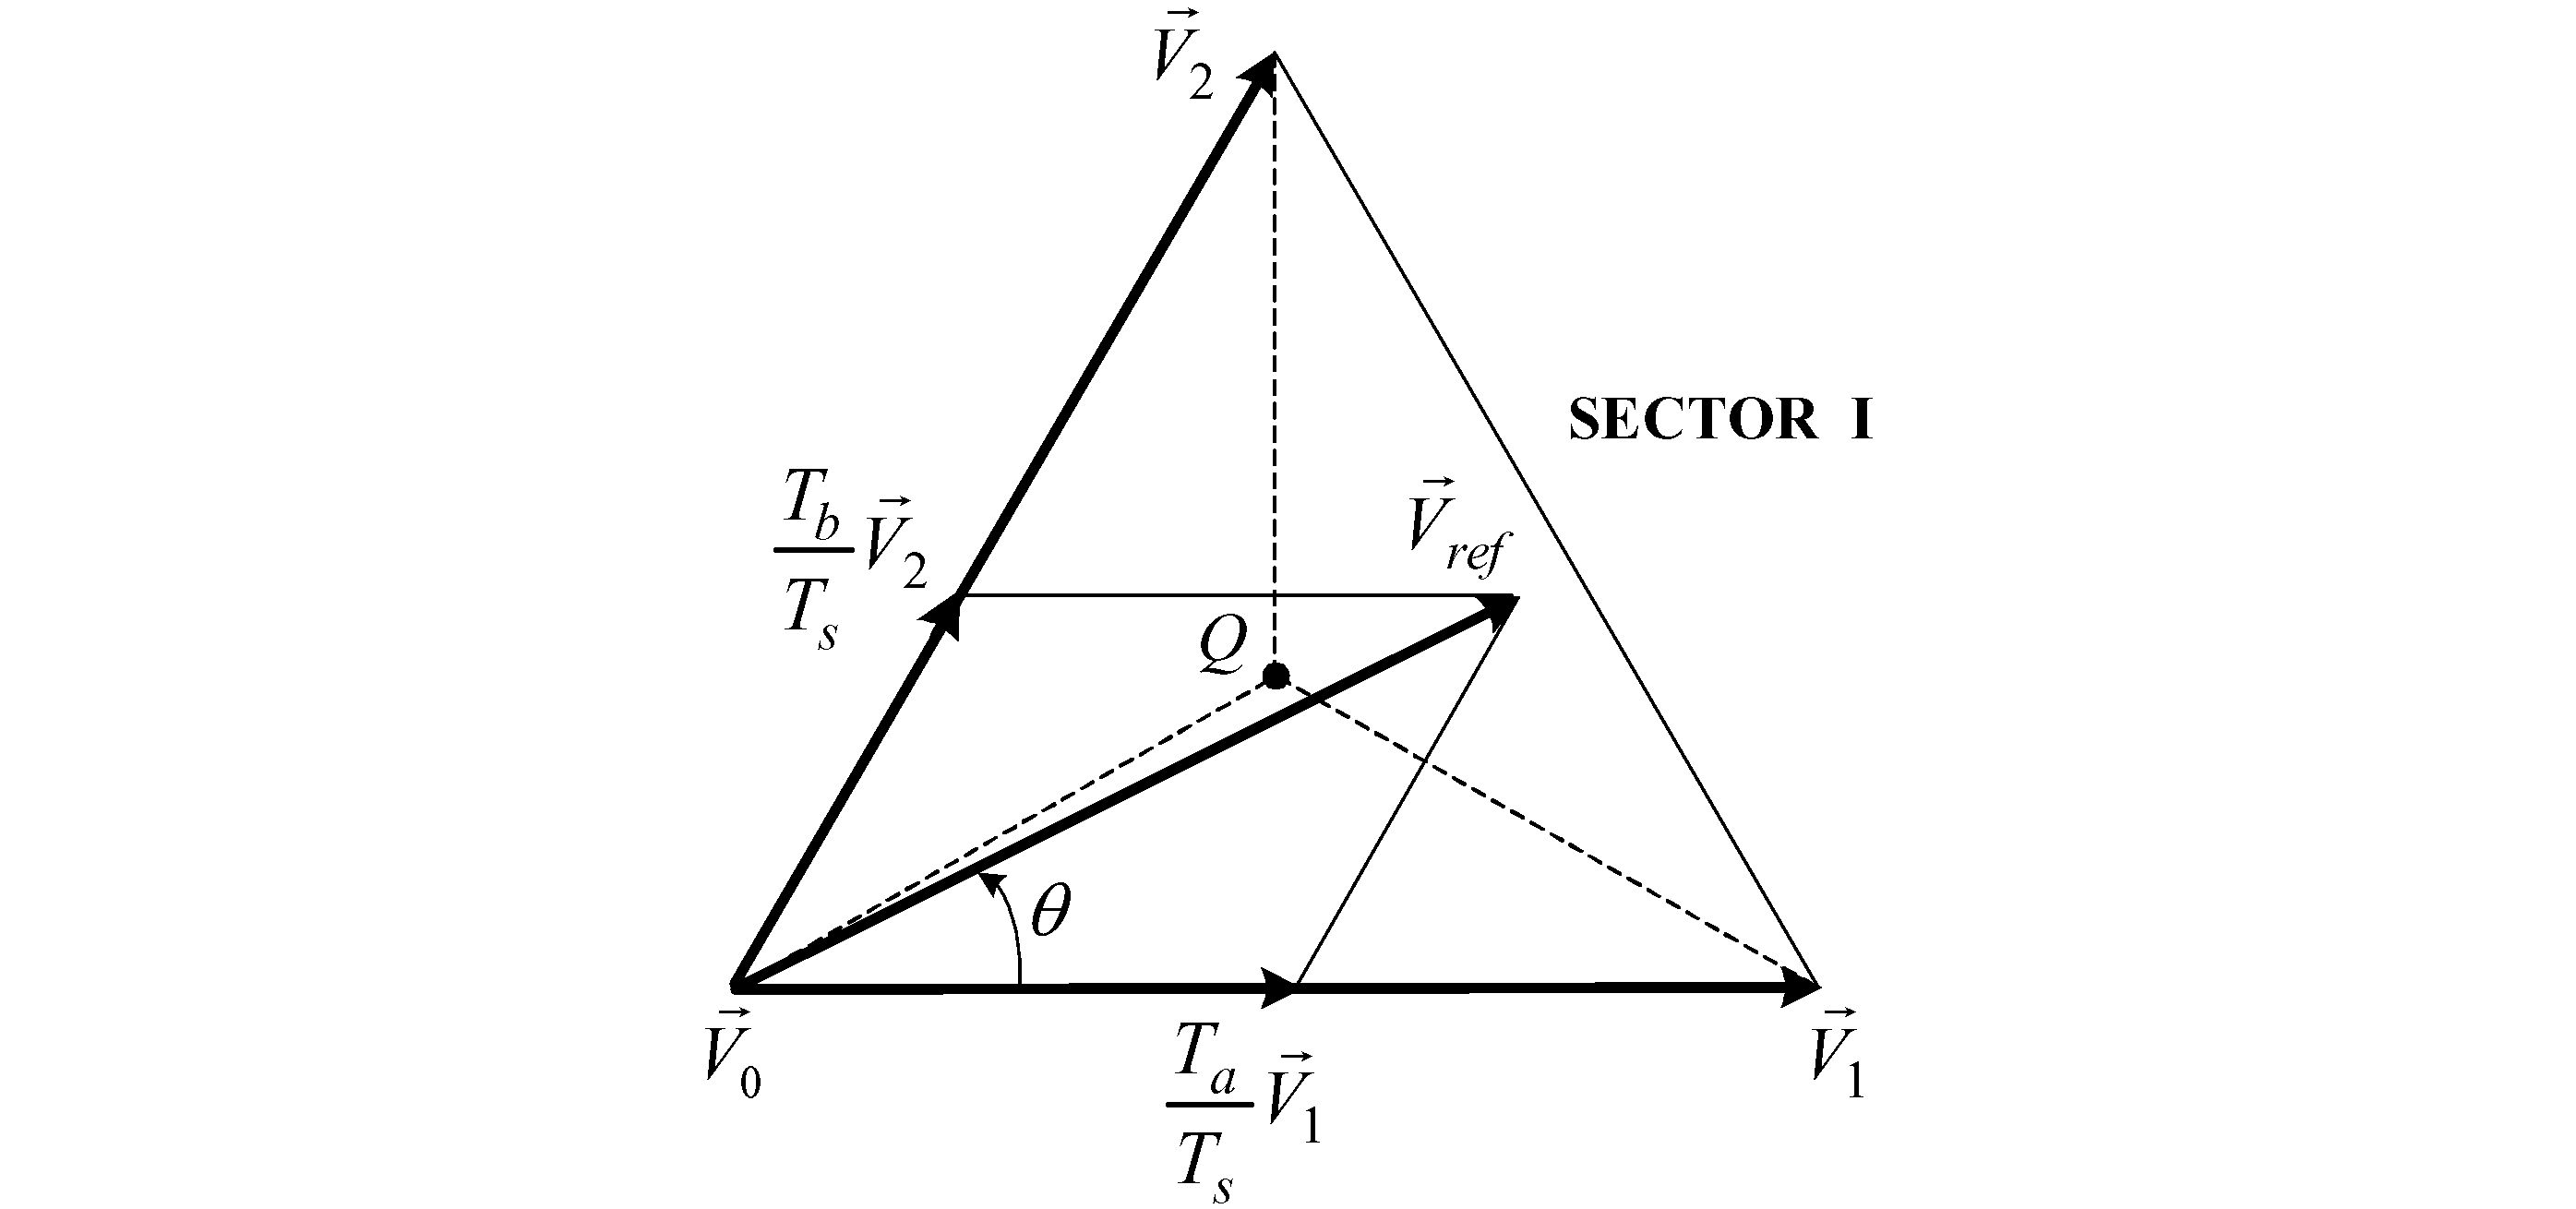
\includegraphics[width=0.6\textwidth]{graficos/img113.jpg}
    \caption{Figure 6.3-2 $\mathbf{V}_{\text{ref}}$ synthesized by $\mathbf{V}_1$, $\mathbf{V}_2$, and $\mathbf{V}_0$.}
    \label{fig:space_vector_synthesis}
\end{figure}
\FloatBarrier

falls into sector I as shown in Fig. 6.3-2, it can be synthesized by \( \mathbf{V}_1 \), \( \mathbf{V}_2 \), and \( \mathbf{V}_0 \). The volt-second balancing equation is
\[
\mathbf{V}_{\text{ref}} T_s = \mathbf{V}_1 T_a + \mathbf{V}_2 T_b + \mathbf{V}_0 T_0 \tag{6.3-10}
\]
where \( T_a \), \( T_b \), and \( T_0 \) are the dwell times for the vectors \( \mathbf{V}_1 \), \( \mathbf{V}_2 \), and \( \mathbf{V}_0 \), respectively. The space vectors in (6.3-10) can be expressed as
\[
\mathbf{V}_1 = \frac{2}{3} V_d, \quad \mathbf{V}_2 = \frac{2}{3} V_d e^{j\frac{\pi}{3}}, \quad \text{and} \quad \mathbf{V}_0 = 0 \tag{6.3-11}
\]

Substituting (6.3-11) into (6.3-10) and then splitting the resultant equation into the real (\(\beta\)-axis) and imaginary (\(\alpha\)-axis) components in the \(\alpha\)-\(\beta\) plane, we have
\[
\text{Re}: V_{\text{ref}}(\cos \theta) T_s = \frac{2}{3} V_d T_a + \frac{1}{3} V_d T_b \tag{6.3-12}
\]
\[
\text{Im}: V_{\text{ref}}(\sin \theta) T_s = \frac{1}{\sqrt{3}} V_d T_b
\]

Solving (6.3-12) together with \( T_s = T_a + T_b + T_0 \) yields
\[
T_a = \frac{\sqrt{3} V_{\text{ref}}}{V_d} \sin\left(\frac{\pi}{3} - \theta\right), \quad T_b = \frac{\sqrt{3} V_{\text{ref}}}{V_d} \sin \theta \quad \text{for} \quad 0 \leq \theta < \frac{\pi}{3} \tag{6.3-13}
\]
\[
T_0 = T_s - T_a - T_b
\]

To visualize the relationship between the location of \( \mathbf{V}_{\text{ref}} \) and the dwell times, let us examine some special cases. If \( \mathbf{V}_{\text{ref}} \) lies exactly in the middle between \( \mathbf{V}_1 \) and \( \mathbf{V}_2 \) (i.e., \(\theta = \frac{\pi}{6}\)), the dwell time \( T_a \) for \( \mathbf{V}_1 \) will be equal to \( T_b \) for \( \mathbf{V}_2 \). When \( \mathbf{V}_{\text{ref}} \) is closer to \( \mathbf{V}_1 \) than \( \mathbf{V}_2 \), \( T_b \) will be greater than \( T_a \). If \( \mathbf{V}_{\text{ref}} \) is coincident with \( \mathbf{V}_2 \), \( T_a \) will be zero. With the head of \( \mathbf{V}_{\text{ref}} \) located right on the central point Q in figure 6.3-2, \( T_a = T_b = T_0 \). The relationship between the \( \mathbf{V}_{\text{ref}} \) location and dwell times is summarized in Table 6.3-3.

Note that although Eq. (6.3-13) is derived when \( \mathbf{V}_{\text{ref}} \) is in sector I, it can also be used when \( \mathbf{V}_{\text{ref}} \) is in other sectors provided that a multiple of \( \pi/3 \) is subtracted from the actual angular displacement \(\theta\) such that the modified angle \(\theta'\) falls into the range between zero and \( \pi/3 \) for use in the equation, that is,
\[
\theta' = \theta - (k-1)\frac{\pi}{3} \quad \text{for} \quad 0 \leq \theta' < \frac{\pi}{3} \tag{6.3-14}
\]
where \( k = 1, 2, \ldots, 6 \) for sectors I, II, \ldots, VI, respectively. For example, when \( \mathbf{V}_{\text{ref}} \) is in sector II, the calculated dwell times \( T_a \), \( T_b \), and \( T_0 \) based on (6.3-13) and (6.3-14) are for vectors \( \mathbf{V}_2 \), \( \mathbf{V}_3 \), and \( \mathbf{V}_0 \), respectively.

\begin{table}[h]
\centering
\caption{Table 6.3-3 $\mathbf{V}_{\text{ref}}$ Location and Dwell Times}
\begin{tabular}{c c c c c c}
\hline
$\mathbf{V}_{\text{ref}}$ Location & $\theta = 0$ & $0 < \theta < \frac{\pi}{6}$ & $\theta = \frac{\pi}{6}$ & $\frac{\pi}{6} < \theta < \frac{\pi}{3}$ & $\theta = \frac{\pi}{3}$ \\ [1em]
Dwell Times: & $T_a > 0$ & $T_a > T_b$ & $T_a = T_b$ & $T_a < T_b$ & $T_a = 0$ \\
& $T_b = 0$ & & & & $T_b > 0$ \\
\hline
\end{tabular}
\end{table}
\FloatBarrier

\subsection*{6.3.4 Modulation Index}

Equation (6.3-13) can be also expressed in terms of modulation index \( m_a \):
\[
T_a = T_{m_a} \sin\left(\frac{\pi}{3} - \theta\right), \quad T_b = T_{m_a} \sin \theta \quad \text{and} \quad T_0 = T_s - T_a - T_b \tag{6.3-15}
\]
where
\[
m_a = \frac{\sqrt{3} V_{\text{ref}}}{V_d} \tag{6.3-16}
\]

The maximum magnitude of the reference vector, \( V_{\text{ref},\text{max}} \), corresponds to the radius of the largest circle that can be inscribed within the hexagon shown in Fig. 6.3-1. Since the hexagon is formed by six active vectors having a length of \( \frac{2}{3} V_d \), \( V_{\text{ref},\text{max}} \) can be found from
\[
V_{\text{ref},\text{max}} = \frac{2}{3} V_d \times \frac{\sqrt{3}}{2} = \frac{V_d}{\sqrt{3}} \tag{6.3-17}
\]

Substituting (6.3-17) into (6.3-16) gives the maximum modulation index:
\[
m_{a,\text{max}} = 1
\]

from which the modulation index for the SVM scheme is in the range of
\[
0 \leq m_a \leq 1 \tag{6.3-18}
\]

The maximum fundamental line-to-line voltage (rms) produced by the SVM scheme can be calculated by
\[
V_{\text{max},SVM} = \sqrt{3} (V_{\text{ref},\text{max}}/\sqrt{2}) = 0.707V_d \tag{6.3-19}
\]

where \( V_{\text{ref},\text{max}}/\sqrt{2} \) is the maximum rms value of the fundamental phase voltage of the inverter.

With the inverter controlled by the SPWM scheme, the maximum fundamental line-to-line voltage is
\[
V_{\text{max,SPWM}} = 0.612V_d
\]
from which
\[
\frac{V_{\text{max,SVM}}}{V_{\text{max,SPWM}}} = 1.155
\]
Equation (6.3-21) indicates that for a given dc bus voltage the maximum inverter line-to-line voltage generated by the SVM scheme is 15.5\% higher than that by the SPWM scheme. However, the use of third harmonic injection SPWM scheme can also boost the inverter output voltage by 15.5\%. Therefore, the two schemes have essentially the same dc bus voltage utilization.

\subsection*{6.3.5 Switching Sequence}

With the space vectors selected and their dwell times calculated, the next step is to arrange switching sequence. In general, the switching sequence design for a given \( \mathbf{V}_{\text{ref}} \) is not unique, but it should satisfy the following two requirements for the minimization of the device switching frequency:

\begin{enumerate}
    \item The transition from one switching state to the next involves only two switches in the same inverter leg, one being switched on and the other switched off.
    \item The transition for \( \mathbf{V}_{\text{ref}} \) moving from one sector in the space vector diagram to the next requires no or minimum number of switchings.
\end{enumerate}

Figure 6.3-3 shows a typical \textit{seven-segment switching sequence} and inverter output voltage waveforms for \( \mathbf{V}_{\text{ref}} \) in sector I, where \( \mathbf{V}_{\text{ref}} \) is synthesized by \( \mathbf{V}_1 \), \( \mathbf{V}_2 \), and \( \mathbf{V}_0 \). The sampling period \( T_s \) is divided into seven segments for the selected vectors. The following can be observed:

\begin{itemize}
    \item The dwell times for the seven segments add up to the sampling period (\( T_s = T_a + T_b + T_0 \)).
    \item Design requirement (a) is satisfied. For instance, the transition from [000] to [POO] is accomplished by turning \( S_1 \) on and \( S_4 \) off, which involves only two switches.
    \item The redundant switching sates for \( \mathbf{V}_0 \) are utilized to reduce the number of switchings per sampling period. For the \( T/4 \) segment in the center of the sampling period, the switching state [PPP] is selected, whereas for the \( T_d/4 \) segments on both sides, the state [000] is used.
    \item Each of the switches in the inverter turns on and off once per sampling period. The switching frequency \( f_{\text{sw}} \) of the devices is thus equal to the sampling frequency \( f_{\text{sp}} \), that is, \( f_{\text{sw}} = f_{\text{sp}} = \frac{1}{T_s} \).
\end{itemize}

\begin{figure}[h]
    \centering
    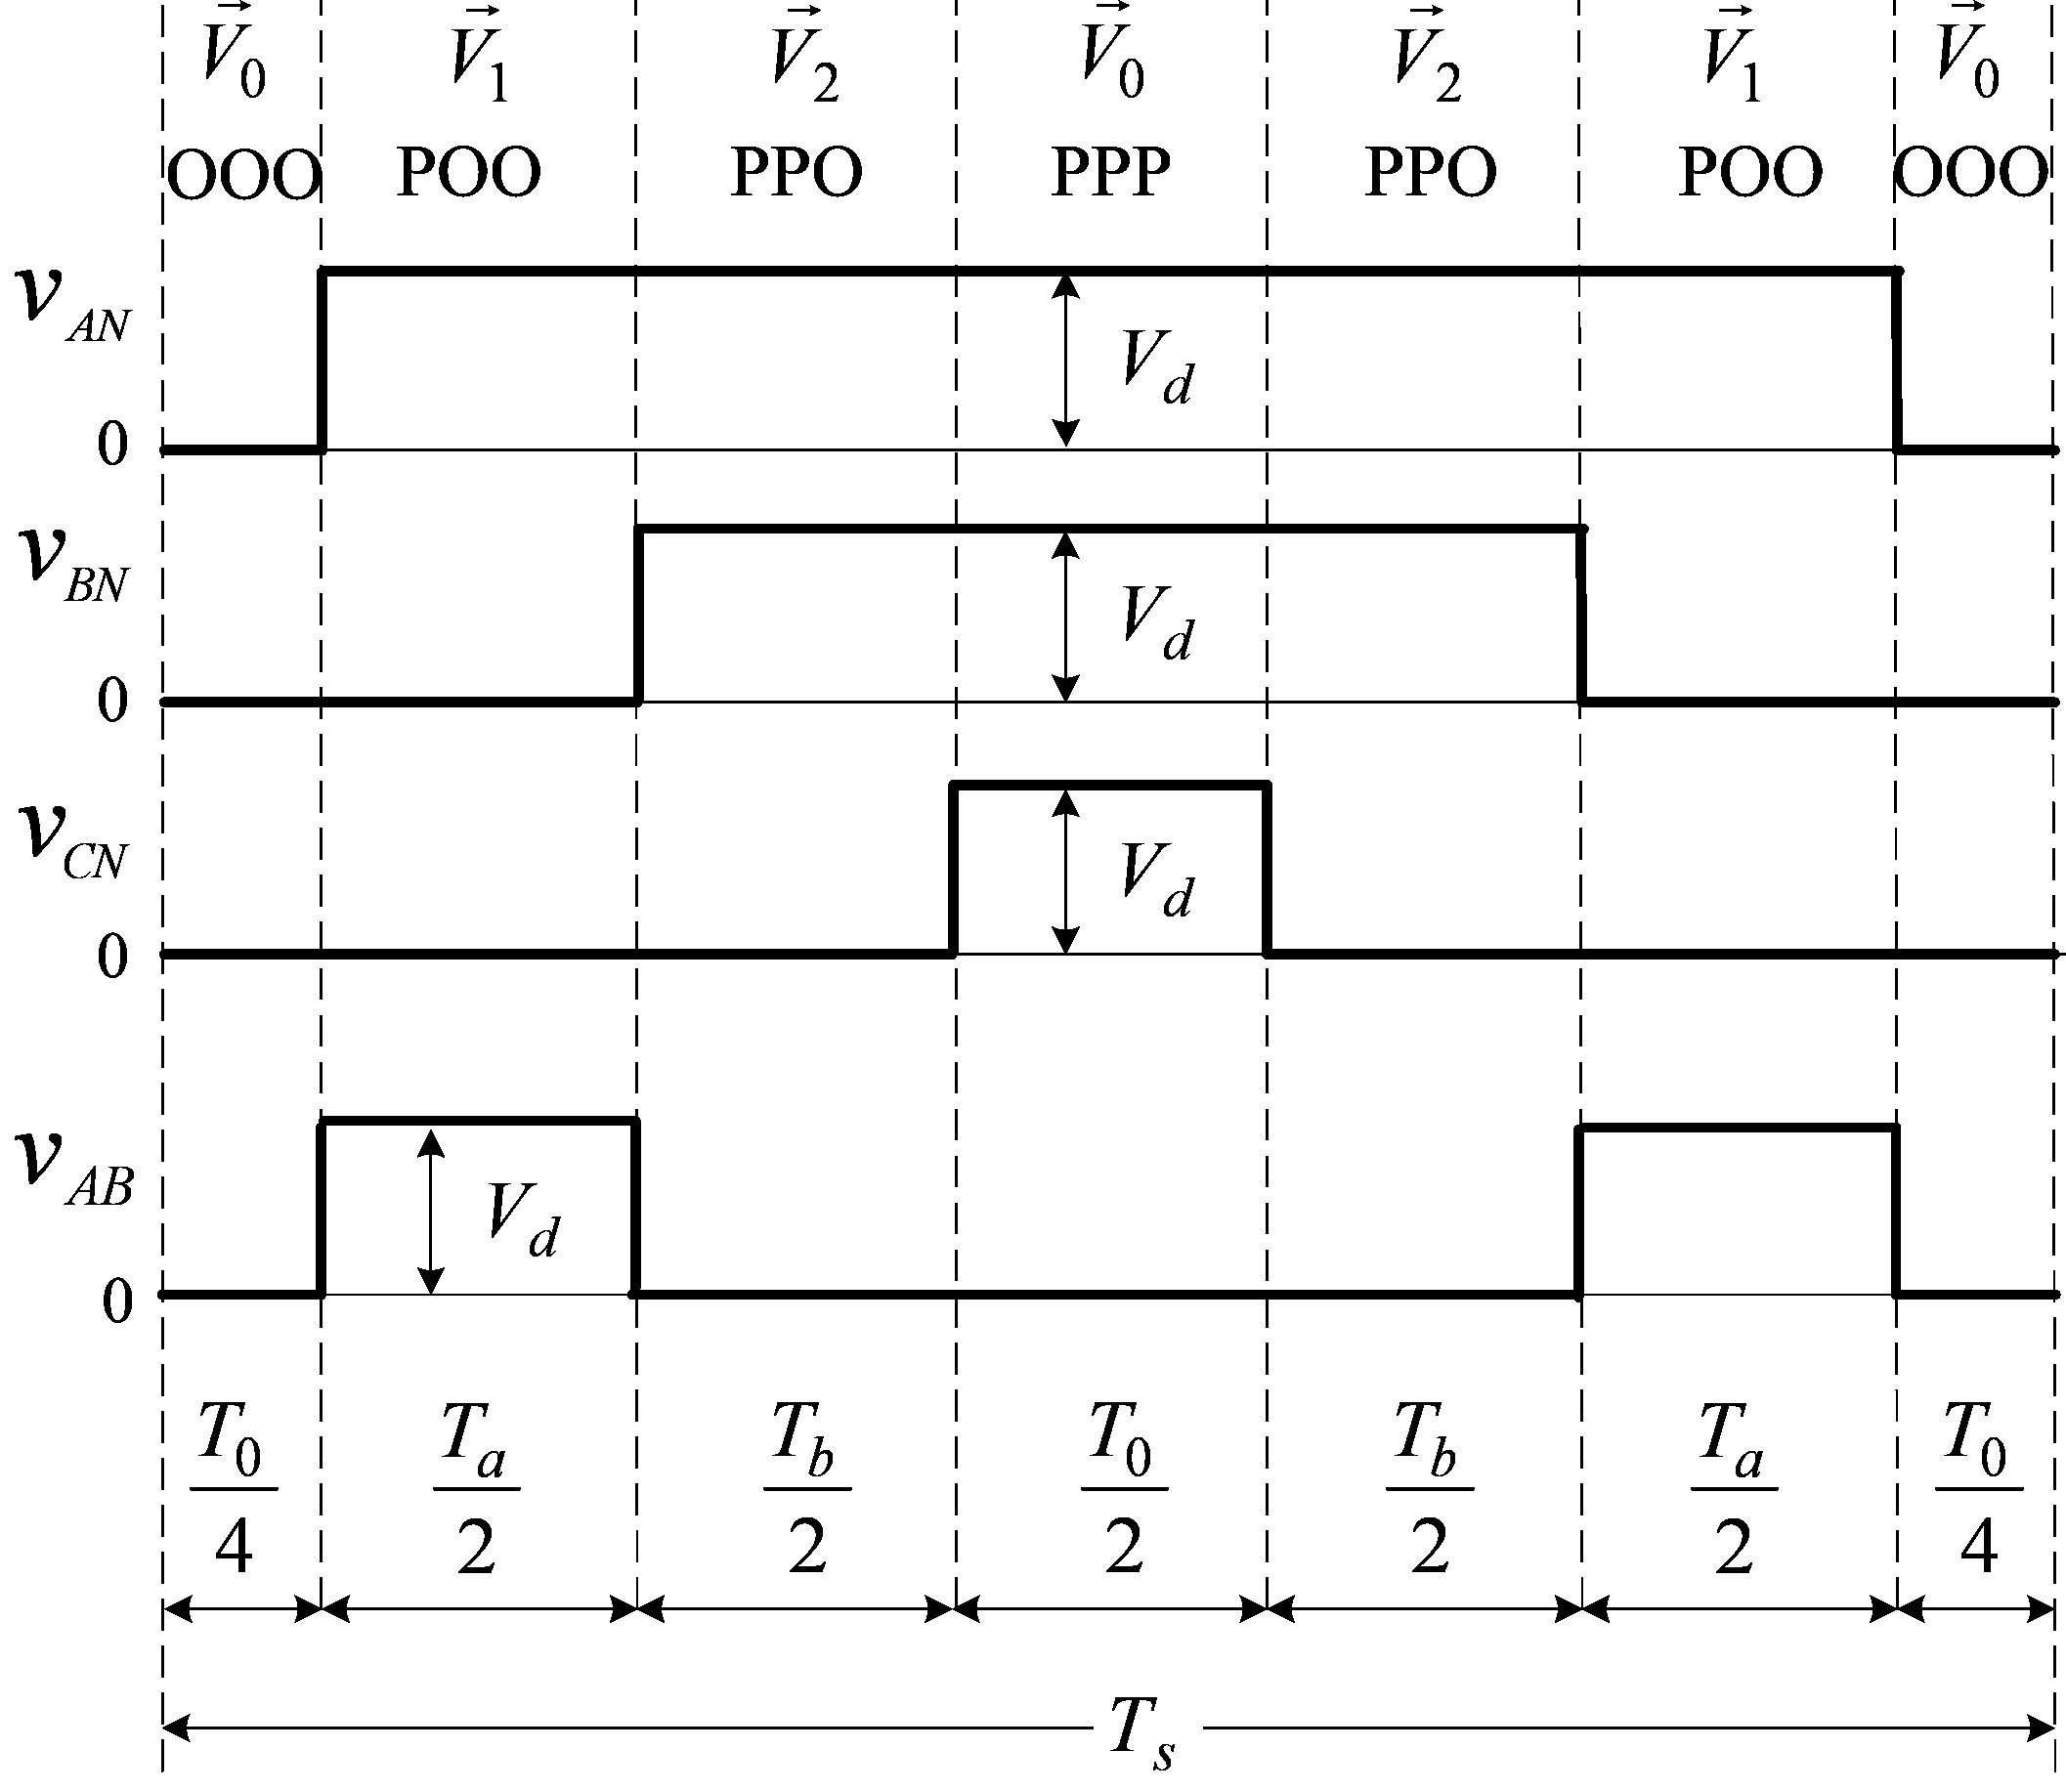
\includegraphics[width=0.6\textwidth]{graficos/img133.jpg}
    \caption{Figure 6.3-3 Seven-segment switching sequence for \( \mathbf{V}_{\text{ref}} \) in sector I.}
    \label{fig:6.3-3}
\end{figure}
\FloatBarrier

Let us now examine a case given in Fig. 6.3-4, where the vectors \( \mathbf{V}_1 \) and \( \mathbf{V}_2 \) in Fig. 6.3-3 are swapped. Some switching state transitions, such as the transition from [000] to [PPO], are accomplished by turning on and off four switches in two inverter legs simultaneously. As a consequence, the total number of switchings during the sampling period increases from six in the previous case to ten. Obviously, this switching sequence does not satisfy the design requirement and thus should not be adopted.

It is interesting to note that the waveforms of \( V_{AB} \) in Figs. 6.3-3 and 6.3-4 produced by two different switching sequences seem different, but they are essentially the same. If these two waveforms are drawn for two or more consecutive sampling periods, we will notice that they are identical except for a small time delay (\( T/2 \)). Since \( T_s \) is much shorter than the period of the inverter fundamental frequency, the effect caused by the time delay is negligible.

Table 6.3-4 gives the seven-segment switching sequences for \( \mathbf{V}_{\text{ref}} \) residing in all six sectors. Note that all the switching sequences start and end with switching state [000], which indicates that the transition for \( \mathbf{V}_{\text{ref}} \) moving from one sector to the next does not require any switchings. The switching sequence design requirement (b) is satisfied.

\subsection*{6.3.6 Spectrum Analysis}

The simulated waveforms for the inverter output voltages and load current are shown in Fig. 6.3-5. The inverter operates under the condition of \( f_1 = 60 \text{ Hz} \), \( T_s = 1/720 \text{ s} \), \( f_{\text{sw}} = 720 \text{ Hz} \), and \( m_a = 0.8 \) with a rated three-phase inductive load. The load power factor is 0.9 per phase. It can be observed that the waveform of the inverter output voltage and the load current are sinusoidal with minimal harmonic distortion.


\end{document}
